\documentclass[10pt,a5paper]{article}
\usepackage[utf8x]{inputenc}
\usepackage[russian]{babel}
\usepackage[OT1]{fontenc}
\usepackage{amsmath}
\usepackage{amsfonts}
\usepackage{amssymb}
\usepackage[left=1.2cm, right=1.2cm, top=1.8cm, bottom=1.8 cm]{geometry}
\usepackage{graphicx}
\graphicspath{{./img/}}

\begin{document}
\begin{titlepage}
	\vspace*{5cm}
	\centering
	{\Huge \scshape \bfseries Астрадь}
\end{titlepage}
\tableofcontents
\newpage

%\section{Небесная механика}


\subsection{Закон всемирного тяготения}
Сила притяжения между двумя телами с массами M и m, 
где $G\approx\ 6.67\cdot \cdot10^{-11}\frac{\text{Н}
\cdot \text{м}^2}{\text{кг}^2}$ --- гравитационная 
постоянная.\begin{equation}
	F=G\frac{Mm}{R^2}
\end{equation}
Потенциал точечной (или сферически симметричной) массы 
$M$ в точке $r$; он равен энергии единичной массы, 
принесенной из бесконечности в эту точку.\begin{equation}
U=-\frac{GM}{r}
\end{equation}
Ускорение свободного падения.\begin{equation}
	g = G \frac{M}{R^2}
\end{equation}
Ускорение свободного падения для тел солнечной системы:
\begin{table}[h!]
\centering
\begin{tabular}{|c|c|c|c|}
\hline 
\textbf{Планета} & $\mathbf{g}$, \textbf{м/c$~^2$} 
& \textbf{Планета} & $\mathbf{g}$, \textbf{м/c$~^2$}\\
\hline
Солнце & 274 & Марс & 3,7\\
\hline
Меркурий & 3,7 & Юпитер & 24,8\\
\hline
Венера & 8,9 & Сатурн & 10,4\\
\hline
Земля & 9,8 & Уран & 8,8\\
\hline
Луна & 1,6 & Нептун & 11,2\\
\hline
\end{tabular}
\end{table}
%\subsection{Закон сохранения энергии и типы орбит}
Для движения тела c массой $m$ в гравитационном  в поле тела 
с массой \linebreak $M\gg m$ со скорость $v$ на расстоянии $r$ от 
гравитационного центра справедливо следующее соотношение: 
\begin{equation}
\frac{m v^2}{2}-\frac{GM m }{r}=E_0,
\end{equation}
где $E_0$ --- постоянная величина, если на тело не действуют
внешние силы кроме силы притяжения к центральному телу, 
равная сумме кинетической и потенциальной энергии тела. Данное равенство принято называть \term{законом сохранения энергии} для тела, движущегося в поле консервативных (потенциальных) сил.

Если $E_0>0$, то траектория тела --- \imp{гипербола}, 
ветви которой асимптотически приближаются к двум прямым. Стоит заметить,
что на бесконечно большом удалении тела с массой $m$ от массивного тела
его скорость остается положительной, так как суммарная энергия $E_0$ 
больше нуля.

Если $E_0=0$, то траектория тела --- \imp{парабола}. При стремлении
расстояния $r$ между телами к бесконечности, скорость тела с массой $m$ 
стремится к нулю.

Отсюда становится очевидно, что на параболической и гиперболический
 траекториях движение тела не ограничено (инфинитно). 

Если $E_0<0$, то траектория тела --- \imp{эллипс}. При 
эллиптической траектории движение ограничено (финитно), так как малое тело
не может бесконечно удалять с неотрицательной скоростью по причине того,
что суммарная энергия меньше нуля.



На Рис.\,\ref{pic:orbits} представлены примеры возможных траекторий тела 
относительно центрального (точка C). При $v_0 > v_{2}$ --- тело движется 
по гиперболе, при $v_0 = v_{2}$ --- по параболе, 
а при $v_0 < v_{2}$ --- по эллипсу.\\

\begin{figure}[h!]
\centering
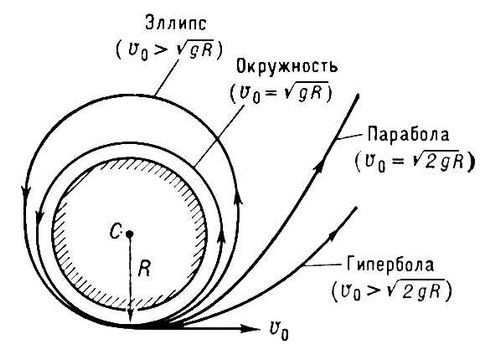
\includegraphics[width = 0.5\textwidth]{Space-speed}
\caption{Возможные траектории тела \label{pic:orbits}}
\end{figure}

\term{Первая космическая скорость} --- минимальная скорость, необходимая для 
того, чтобы маломассивное тело стало искусственным спутником центрального тела.
\begin{equation}v_1=\sqrt{\frac{GM}{R}}
\end{equation}
где $M$ --- масса массивного тела. Отсюда несложно получить выражение для
скорости искусственного небесного тела на высоте 
$h$.\begin{equation}v_h=\sqrt{\frac{GМ}{R+h}}=\sqrt{\frac{gR^2}{R+h}}
\end{equation}\\

\term{Параболическая} или \term{вторая космическая скорость} --- 
минимальная скорость, необходимая для того, чтобы маломассивное тело преодолело 
гравитационное притяжение центрального тела и покинуло замкнутую орбиту вокруг 
последнего. Выражение для которой имеет следующий вид:\begin{equation}
v_{2}=\sqrt{\frac{2GM}{r}}
\end{equation}

Для стабильной системы, частный случай~--- тело на круговой орбите, справедлива 
\term{теорема о вириале}:
\begin{equation}
2 \langle T\rangle 
= -\sum _{{k=1}}^{N}\langle {F}_{k}\cdot {r}_{k}\rangle 
= \langle U \rangle
\end{equation}

Где $\langle T\rangle$ --- средняя полная кинетическая энергия, $F_k$ --- сила, 
действующая на $k$-ю частицу. Другими словами, удвоенная средняя полная 
кинетическая энергия $T$ равна средней полной потенциальной энергии $U$. 

Применяя теорему о вириале для тела, обращающегося по круговой орбите можно 
получить выражения для первой космической скорость.

\begin{table}[h!]
\centering
\begin{tabular}{|c|c|c|}
\hline
\textbf{Планета} & $\mathbf{v_1}$,~\textbf{км/c} & 
$\mathbf{v_2}$,~\textbf{км/c}\\
\hline
Солнце & 436,8 & 617,7\\
\hline
Меркурий & 3,0 & 4,3\\
\hline
Венера & 7,4 & 10,5\\
\hline
Земля & 7,9 & 11,2\\
\hline
Луна & 1,7 & 2,4\\
\hline
Марс & 3,5 & 5,0\\
\hline
Юпитер & 42,0 & 59,5\\
\hline
Сатурн & 25,1 & 35,5\\
\hline
Уран & 15,0 & 21,3\\
\hline
Нептун & 16,6 & 23,5\\
\hline
\end{tabular}
\caption{$v_1$ и $v_2$ на некоторых телах Солнечной системы}
\end{table}





%\subsection{Законы Кеплера}
{\bfseries I-ый закон:} Все планеты движутся по 
эллиптическим орбитам, в одном из фокусов которых 
находится Солнце.\\
{\bfseries II-ой закон:} Радиус-вектор планеты за 
равные промежутки времени заметает равные площади.
\begin{equation}
\frac{dS}{dt}=const
\end{equation}
\begin{figure}[h!]
\begin{minipage}[b]{0.5\textwidth}
\centering
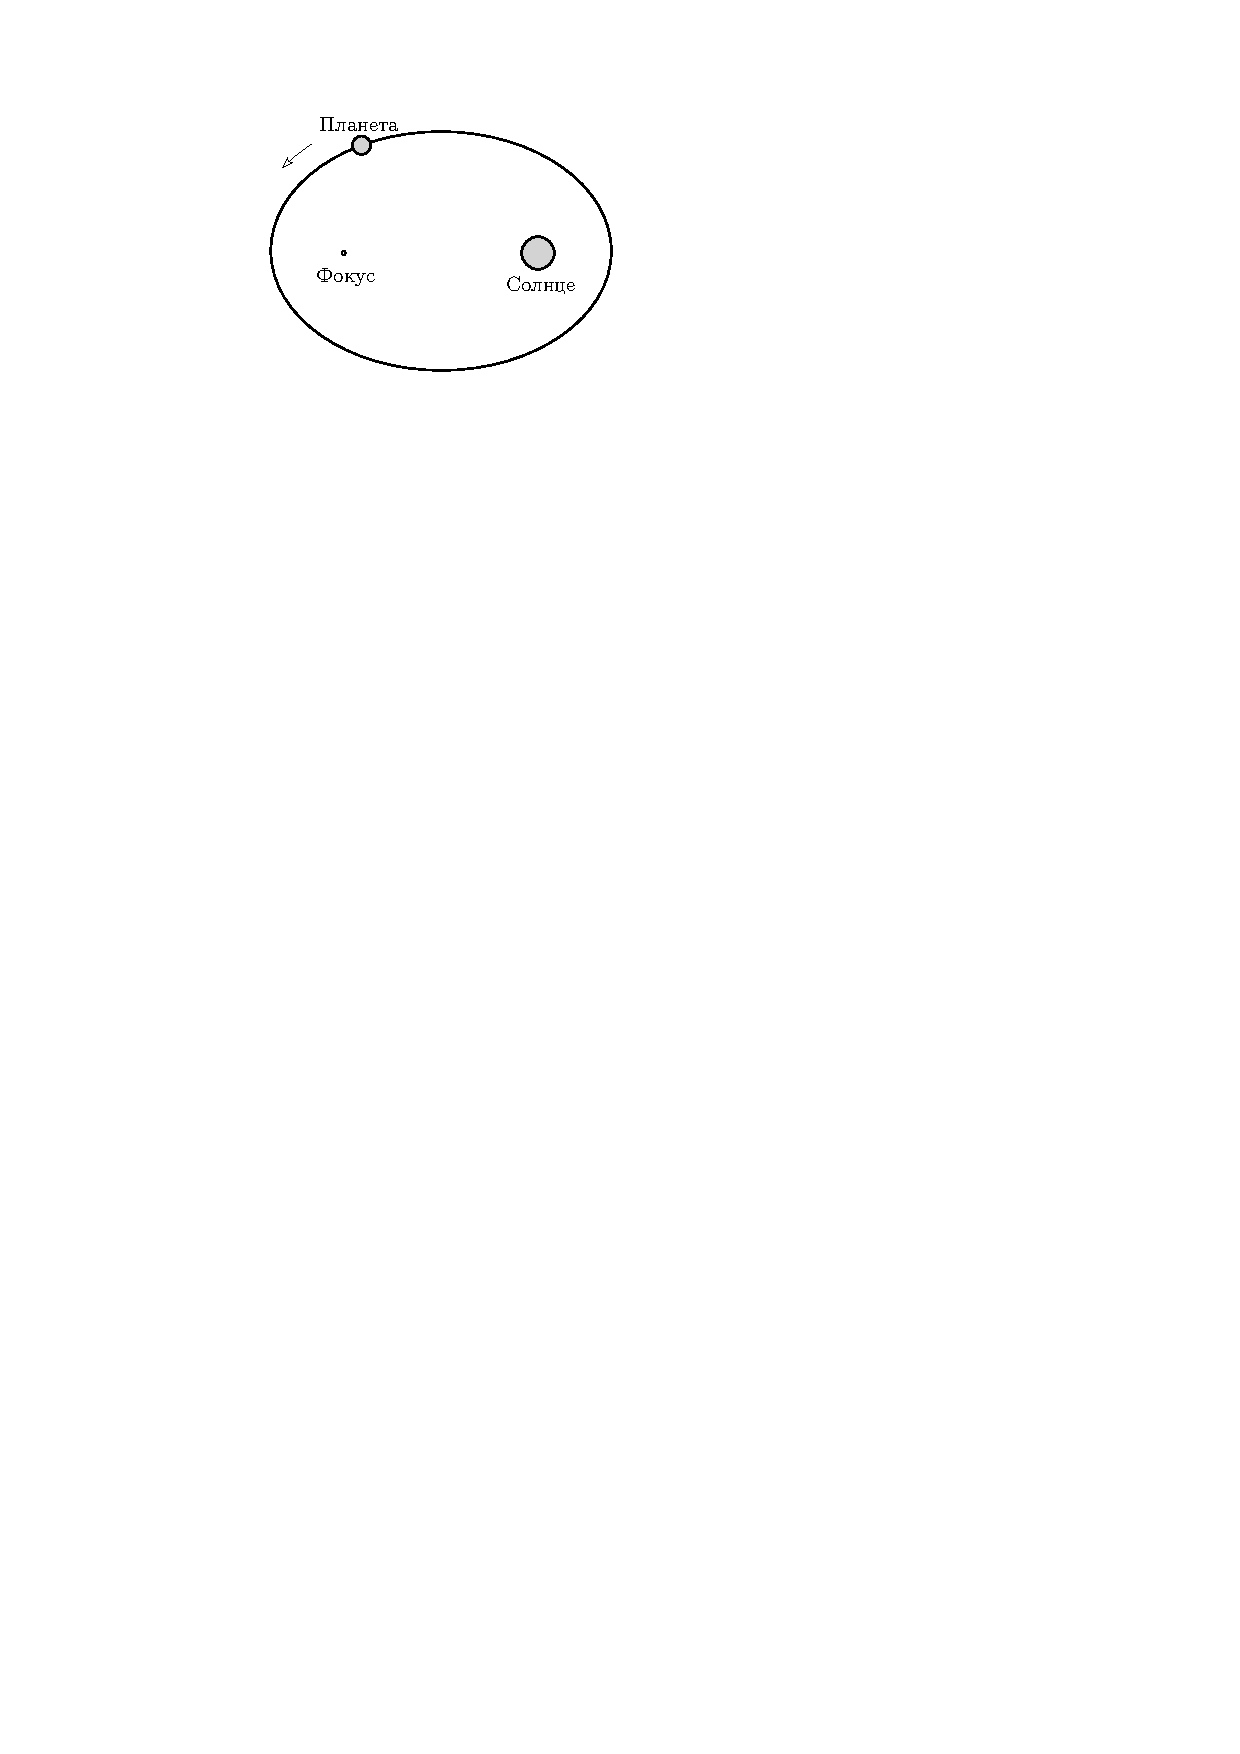
\includegraphics[width = 0.7\textwidth]{first-kepler}
\caption{Первый закон Кеплера}
\end{minipage}
\begin{minipage}[b]{0.5\textwidth}
\centering
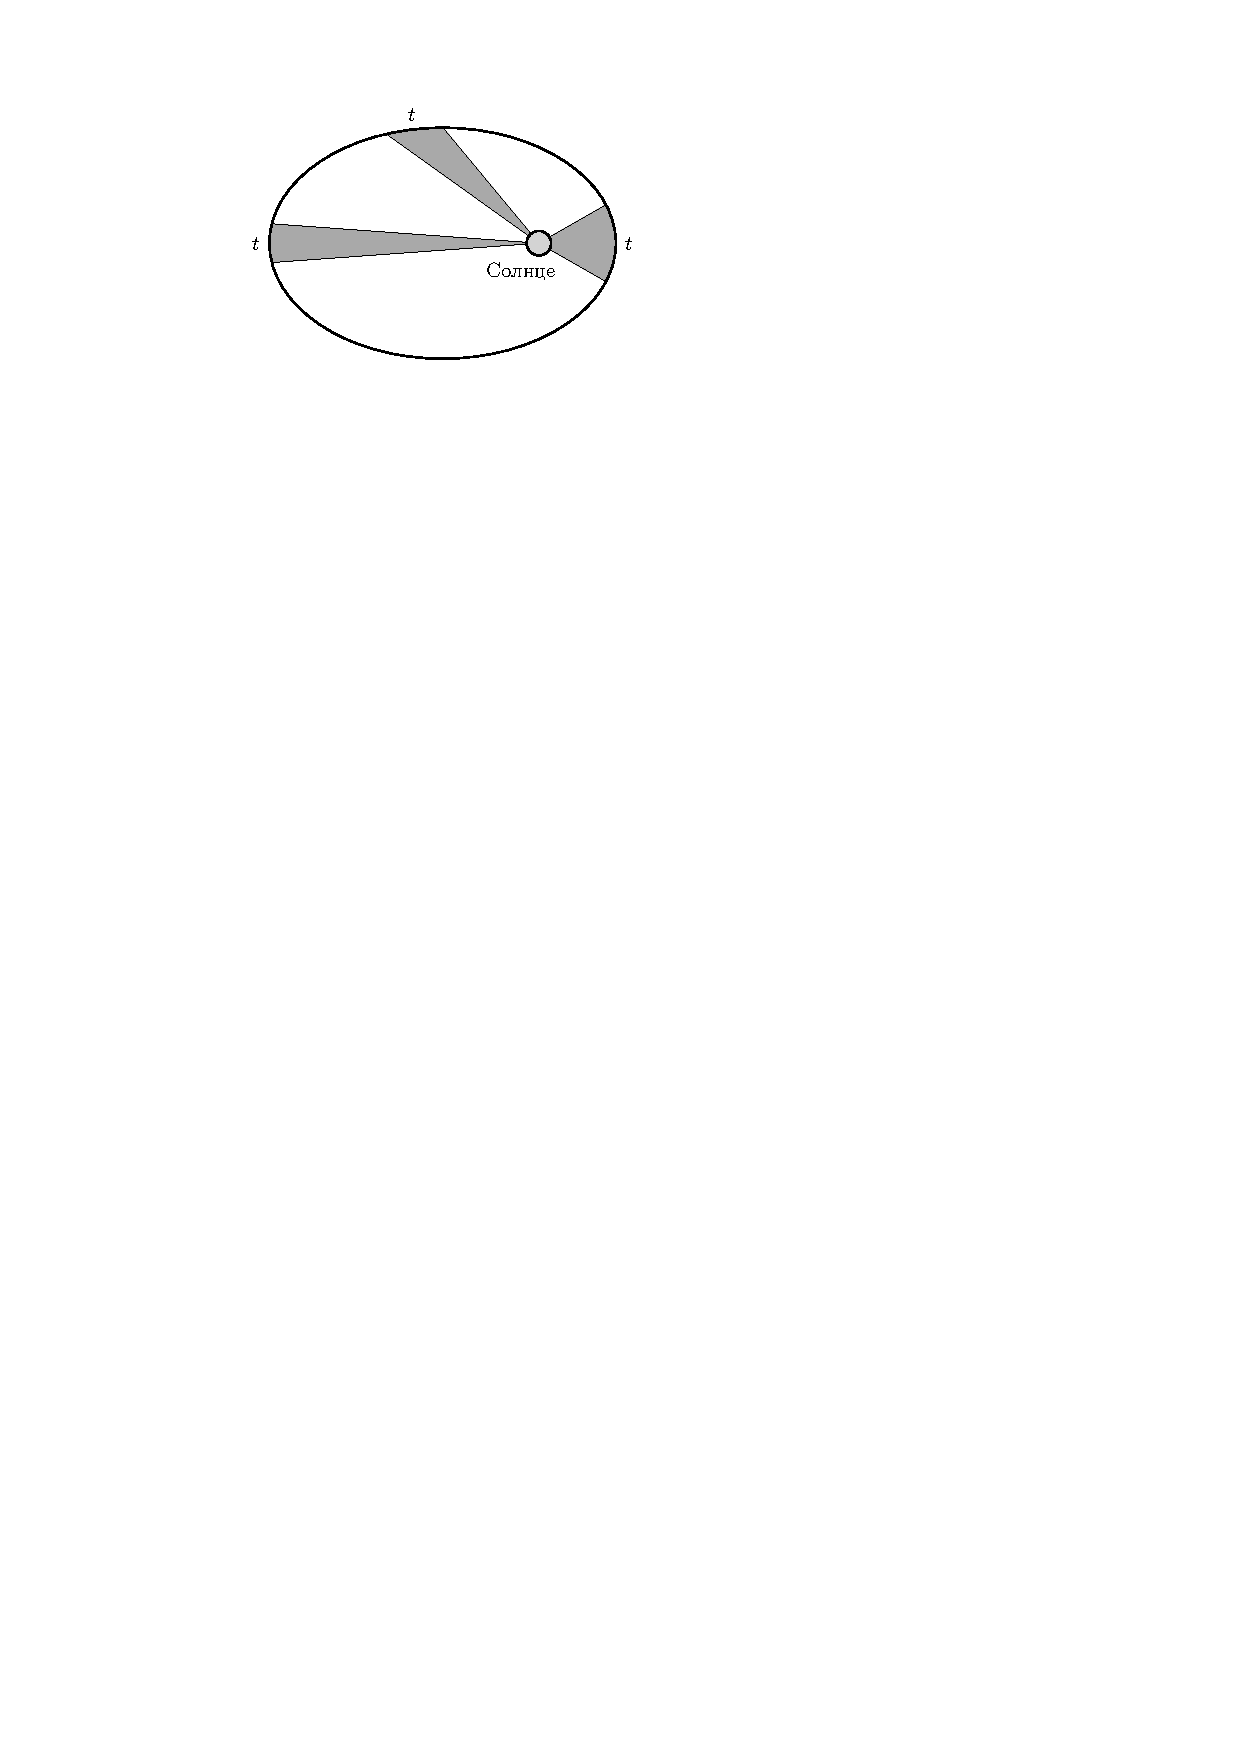
\includegraphics[width = 0.81\textwidth]{second-kepler}
\caption {Второй закон Кеплера}
\end{minipage}
\end{figure}

{\noindent \bfseries III-ий закон:} Квадраты периодов обращения планет 
относятся, как кубы больших полуосей их орбит.
\begin{equation}
\frac{T^2_1}{T^2_2}=\frac{a^3_1}{a^3_2},
\end{equation}
где $a$ --- большая полуось, $T$ --- период обращения.
Обобщённый Ньютоном III-ий закон имеет следующий вид:
\begin{equation}
\frac{T^2_1(M_1+m_1)}{T^2_2(M_2+m_2)}=\frac{a^3_1}{a^3_2}
\end{equation}
или, что эквивалентно, \begin{equation}
	\frac{T^2}{a^3}=\frac{4\pi^2}{G(M+m)},
\end{equation}
где $M_1$ и $M_2$ --- массы центральных тел, $m_1$ и 
$m_2$ --- массы обращающихся вокруг них тел. Так как массы планет 
$m$ много меньше массы звезды $M$, то $M + m \simeq M$.
%\subsection{Первая, вторая и третья космические скорости} 

\bfseries Первая космическая скорость \mdseries --- минимальная скорость, необходимая для того, чтобы маломассивное тело стало искусственным спутником центрального тела.
$$v_1=\sqrt{\frac{GM}{R}}$$
Где $M$ --- масса массивного тела.

\bfseries Вторая космическая скорость \mdseries --- минимальная скорость, необходимая для того, чтобы маломассивное тело преодолело гравитационное притяжение центрального тела и покинуло замкнутую орбиту вокруг последнего. 
$$v_2=v_p=\sqrt{2gR}=\sqrt{\frac{2GM}{R}}=\sqrt{2}v_1$$
$v_1$ и $v_2$ на некоторых телах Солнечной системы:
\begin{table}[h!]
\centering
\begin{tabular}{|c|c|c|}
\hline
\textbf{Планета} & $\mathbf{v_1}$,\textbf{км/c} & $\mathbf{v_2}$,\textbf{км/c}\\
\hline
Солнце & 436,8 & 617,7\\
\hline
Меркурий & 3,0 & 4,3\\
\hline
Венера & 7,4 & 10,5\\
\hline
Земля & 7,9 & 11,2\\
\hline
Луна & 1,7 & 2,4\\
\hline
Марс & 3,5 & 5,0\\
\hline
Юпитер & 42,0 & 59,5\\
\hline
Сатурн & 25,1 & 35,5\\
\hline
Уран & 15,0 & 21,3\\
\hline
Нептун & 16,6 & 23,5\\
\hline
\end{tabular}
\end{table}

Скорость искусственного небесного тела на высоте $h$.$$v_h=\sqrt{\frac{GМ}{R+h}}=\sqrt{\frac{gR^2}{R+h}}$$

\bfseries Третья космическая скорость \mdseries --- минимальная скорость, которую необходимо придать находящемуся вблизи поверхности Земли телу, что-бы оно могло преодолеть гравитационное притяжение Земли и Солнца и покинуть пределы Солнечной системы.
$$v_3=\sqrt{(\sqrt{2}-1)^2v^2_1+v^2_2}$$ 
%\subsection{Движение по орбите}

\textit{Закон сохранения момента импульса} ---  векторная сумма всех моментов импульса относительно выбранной оси для замкнутой системы тел, которая остается постоянной, пока на систему не воздействуют внешние силы:
\begin{equation}
\vec{r} \cdot m\vec{v}=const  
\end{equation}

Следствием закона сохранения момента импульса и закона сохранения энергиии является        \textit{ интеграл энергии} (скорость в точке орбиты, удалённой на расстояние $r$ от центрального тела, где $M$ --- масса центрального тела):
\begin{equation}v=\sqrt{GM\left(\frac2r - \frac1a\right)}
\end{equation}

При подстановке расстояний ($r$) апоцентра или перицентра интеграл энергии принимает следующий вид:
\begin{equation}v_{\text{аф}}=\sqrt{\frac{GM}{a}} \sqrt{\frac{1-e}{1+e}}
\end{equation}
\begin{equation}v_{\text{пер}}=\sqrt{\frac{GM}{a}}\sqrt{\frac{1+e}{1-e}}
\end{equation}

При использовании уравнения эллипса в полярных координатах значение скорости можно определить по следующей формуле, где $\nu$ --- истинная аномалия, $p$ --- фокальный параметр:
\begin{equation}v=\sqrt{\frac{GM}{p}\cdot(1+2e\nu+e^2)}
\end{equation}

%\subsection{Синодический период}

\textbf{Синодический период} --- промежуток времени между двумя последовательными одноимёнными конфигурациями планеты или Луны. Период смены фаз Луны равен её синодическому периоду.

$S$ --- синодический период. $T$ --- сидерический период. $E$ --- сидерический период обращения Земли.

\textit{Относительная угловая скорость} планеты или скорость углового смещения равна разности скоростей углового перемещения планет по орбите. Отсюда выводятся следующие формулы:

Для внешних планет:
\begin{equation}\frac1S=\frac1E-\frac1T
\end{equation}

Для внутренних планет:
\begin{equation}\frac1S=\frac1T-\frac1E
\end{equation}

В случае, если тело обращается по орбите в протвоположную сторону, то связь между синодическим и сидерическим периодами тела выглядит следующим образом:
\begin{equation}\frac1S=\frac1E+\frac1T
\end{equation}
%\subsection{Конфигурации планет}
\begin{center}
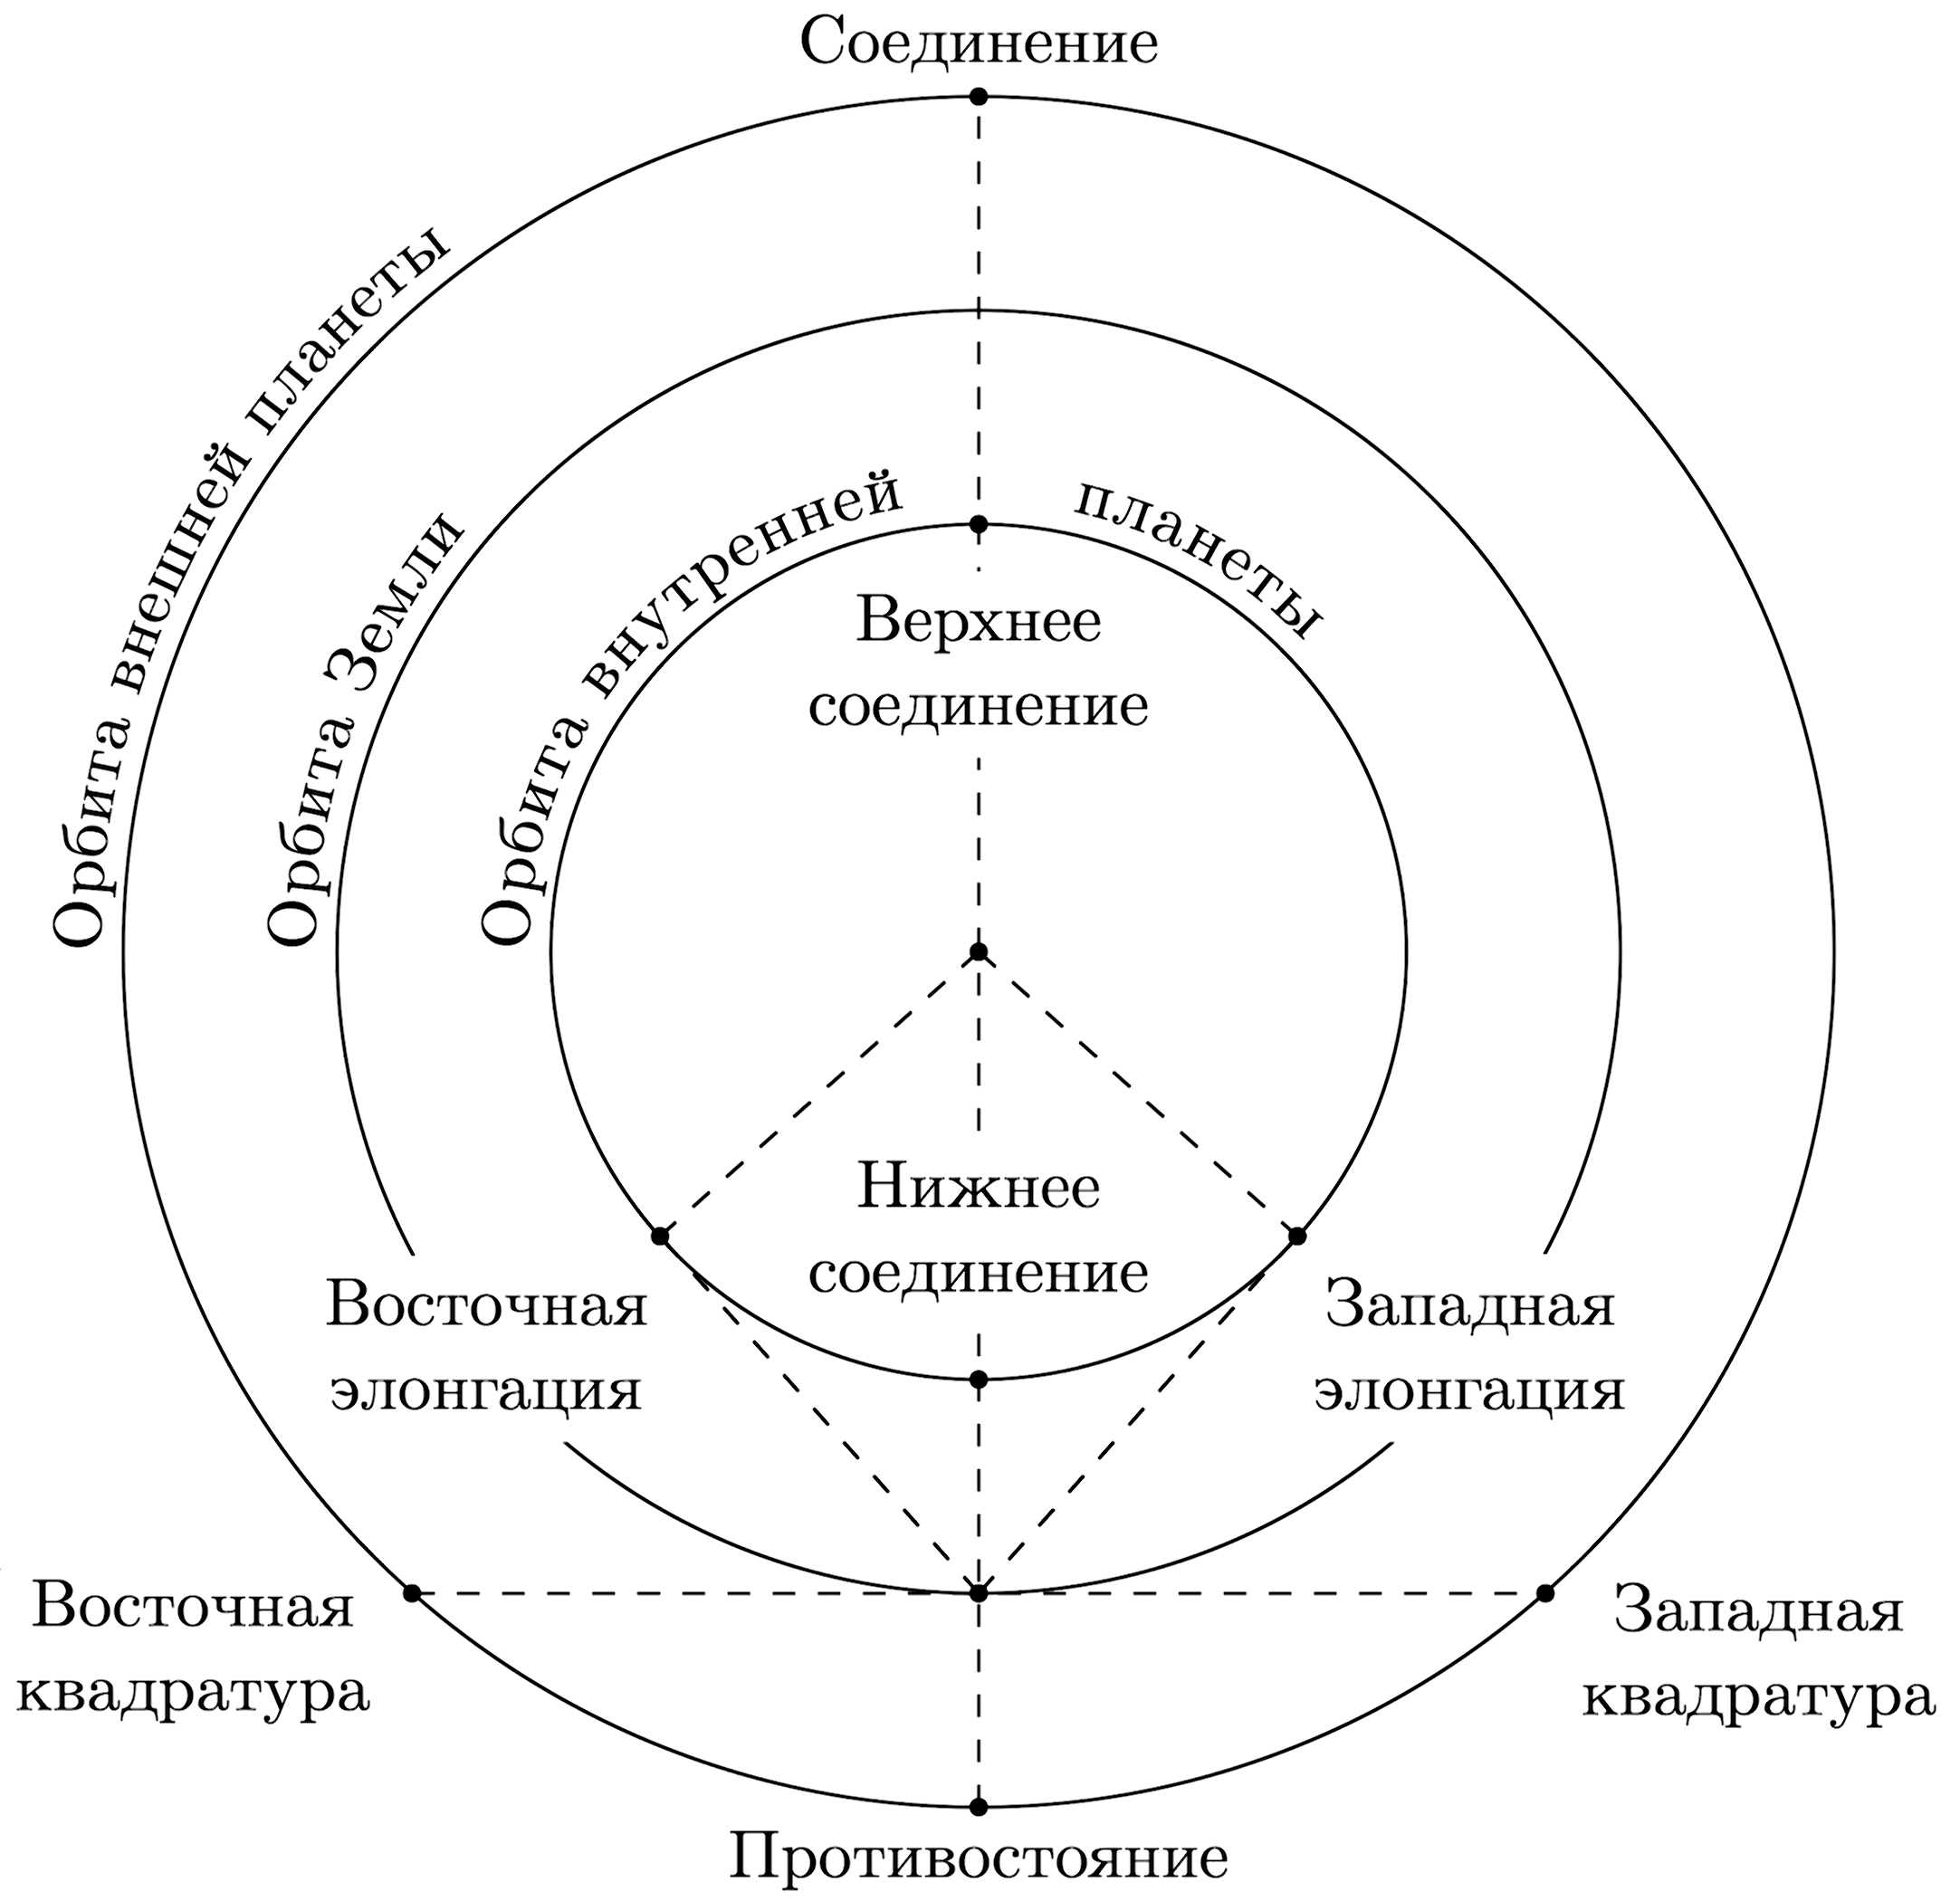
\includegraphics[scale=0.571]{planet-config}
\begin{figure}[h!]
\caption{Конфигурации планет}
\end{figure}
\end{center}
%\subsection{Кеплеровы элементы орбиты}

\textbf{Кеплеровы элементы} --- шесть элементов орбиты, определяющие положение небесного тела в пространстве в задаче двух тел:
\begin{enumerate}
\item Большая полулось($a$);
\item Эксцентриситет ($e$);
\item Наклонение($i$);
\item Аргумент перицентра($\omega$);
\item Долгота восходящего узла($\Omega$);
\item Средняя аномалия ($M_0$);
\end{enumerate}
Первые два определяют форму орбиты, третий, четвёртый и пятый — ориентацию плоскости орбиты по отношению к базовой системе координат, шестой — положение тела на орбите (Рис.5).

\textbf{Наклонение} --- небесного тела — это угол между плоскостью его орбиты и плоскостью эклиптики.
\textbf{Аргумент перицентра} --- угол между направлениями из притягивающего центра на восходящий узел орбиты и на перицентр.

\textbf{Долгота восходящего узла} --- угол в плоскости эклиптики между направлением на точку весеннего равноденствия и восходящий узел орбиты. Отсчитывается против часовой стрелки от направления на точку весеннего равноденствия.

\textbf{Средняя аномалия} для тела, движущегося по невозмущённой орбите --- произведение его среднего движения и интервала времени после прохождения перицентра.

\textbf{Узлы орбиты} --- точки пересечения орбиты и плоскости эклиптики.

\textbf{Восходящий узел} --- точка, в которой тело пересекает плоскость эклиптики при движении в северноим направлении, а \textbf{нисходящий} --- в южном.

\textbf{Истинная аномалия ($\nu$)} --- угол между радиус вектором и направлением на перицентр.
\begin{center}
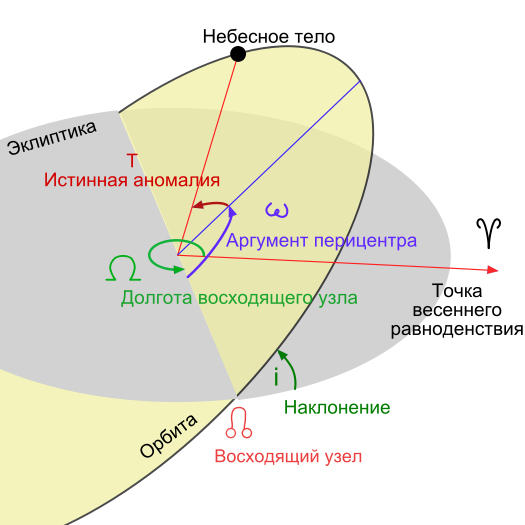
\includegraphics[scale=0.31]{Orbit-elem}
\begin{figure}[h!]
\caption{Кеплеровы элементы орбиты}
\end{figure}
\end{center}
%\subsection{Фазы планет и спутников}

\bfseries Фазой \mdseries планеты (cпутника) называется отношение площади освещённой  части видимого диска ко всей его площади.
Фаза считается по следующей формуле:
\begin{equation}\Phi=\frac{1+\cos\phi}{2}=\cos^2\frac{\phi}{2}
\end{equation}
Где $\phi$ --- \textbf{фазовый угол} --- угол между лучом света, падающим от Солнца на планету, и лучом, отразившимся от неё в сторону наблюдателя (Рис.6). Фаза изменяется от 0 до 1.
\begin{center}
\includegraphics[width = 0.6\textwidth]{phase-angle}
\begin{figure}[h!]
\caption{Фазовый угол}
\end{figure}
\end{center}


%\subsection{Специальная теория относительности. Аберрация}

Обычно в СТО рассматриваются две инерциальные системы $S$ и $S'$. Время и координаты некоторого события, измеренные относительно системы $S$, обозначаются как $(t, x, y, z)$, а координаты и время этого же события, измеренные относительно системы $S'$, как $(t', x', y', z')$. Удобно считать, что координатные оси систем параллельны друг другу, и система $S'$ движется вдоль оси $x$ системы $S$ со скоростью $v$. Одной из задач СТО является поиск соотношений, связывающих $(t', x', y', z')$ и $(t, x, y, z)$, которые называются \textit{преобразованиями Лоренца}. Общий вид преобразований Лоренца в векторном виде, когда скорость систем отсчёта имеет произвольное направление:

\begin{equation}
t'=\gamma\cdot \left(t-\frac{\mathbf{rv}}{c^2}\right),
\end{equation}
\begin{equation}
\mathbf{r'}=r-\gamma vt+(\gamma-1)\cdot\frac{(\mathbf{rv})\mathbf{v}}{v^2},
\end{equation}
где  $\gamma=1/{\sqrt {1-\mathbf {v} ^{2}/c^{2}}}$, $\mathbf{r}$ и $\mathbf{r'}$ --- радиус-векторы события относительно систем $S$ и $S'$.

Если сориентировать координатные оси по направлению относительного движения инерциальных систем и выбрать это направление в качестве оси $x$, то преобразования Лоренца примут следующий вид: 
\begin{equation}
t'=\frac{t-\frac{v}{c^2}x}{\sqrt{1-\frac{v^2}{c^2}}},\quad\text{  } x'=\frac{x-vt}{\sqrt{1-\frac{v^2}{c^2}}},\quad\text{  } y'=y,\quad\text{  } z'=z,
\end{equation}
где $c$ --- скорость света.

 При скоростях много меньше скорости света $(v\ll c)$ преобразования Лоренца переходят в \textit{преобразования Галилея}:
\begin{equation}
 t'=t,\quad\text{  } x'=x-vt,\quad\text{  }  y'=y,\quad\text{  }  z'=z
\end{equation}
 
\textbf{Аберрация} --- явление, состоящее в том, что движущийся наблюдатель видит светило не в том направлении, в котором он видел бы его в тот же момент, если бы находился в покое, причём смещается светило в сторону движения наблюдателя. Происходит это из-за конечности скорости света и из-за изменения системы отсчёта для наблюдателя.  
Угол аберрационного смещения можно найти по следующей формуле:
\begin{equation}\sigma=\frac{v}{c}\sin\theta,
\end{equation}
где $v$ --- скорость наблюдателя, $\theta$ --- угол между направлением вектора скорости наблюдателя и направлением на объект. 
%\subsection{Приливы и отливы}

Приливы и отливы --- периодические вертикальные колебания уровня океана или моря, являющиеся результатом как изменения положения Луны, так Солнца. Хотя силы тяготения Солнца почти в 200 раз больше, чем силы тяготения Луны, приливные силы, порождаемые Луной, почти вдвое больше порождаемых Солнцем. Это происходит из-за того, что приливные силы зависят не от величины гравитационного поля, а от степени его неоднородности. Высота приливов зависит от взаимного расположения Луны и Солнца. Наибольший прилив, когда приливообразующие силы Луны и Солнца действуют вдоль одного направления, а наименьший прилив, когда приливообразующие силы Луны и Солнца действуют под прямым углом друг к другу.

Ускорение в центре Земли($T$) считется по следующей формуле: \begin{equation}\omega_T=\frac{GM}{r^2},
\end{equation}

Где $M$ --- масса Луны, $r$ --- расстояние между центрами Земли и Луны. Ускорения в точках A и B равны:
\begin{equation}\omega_A=\frac{GM}{(r-R)^2} \text{ и } \omega_B=\frac{GM}{(r+R)^2},
\end{equation}

Где $R$ --- радиус Земли. Ускорение точки A относительно точки T равно:
\begin{equation}\omega_A-\omega_T=\omega_T\frac{2rR-R^2}{(r-R)^2},
\end{equation}

Так как $R\ll r$, то \begin{equation}\omega_A-\omega_T=\omega_T\frac{2R}{r}
\end{equation}

Под действием лунного притяжения водная оболочка Земли принимает форму эллипсоида, который вытянут по направлению к Луне. Близ точек $A$ и $B$ будет прилив, а у точек $F$ и $D$ --- отлив (Рис.\ref{Ebb_flow}).
\begin{center}
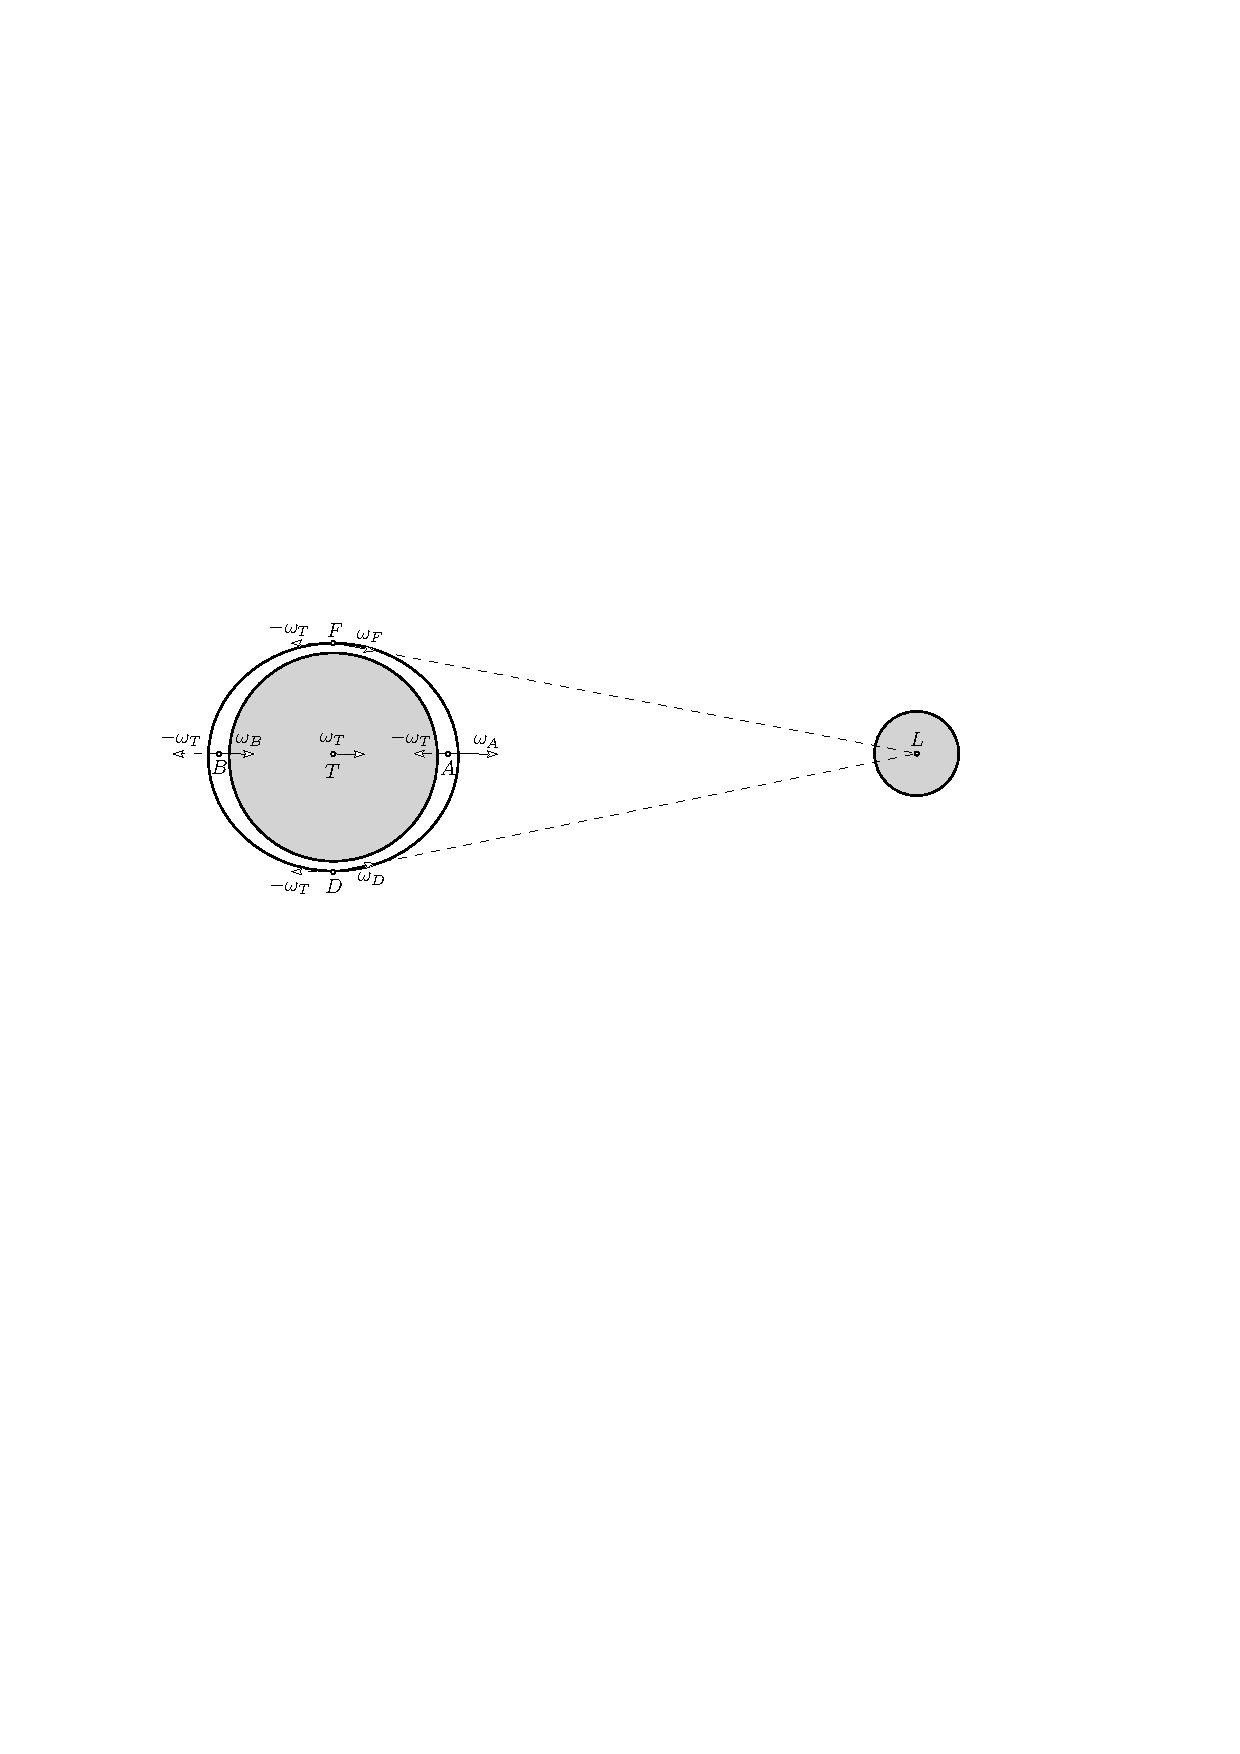
\includegraphics[width = 1\textwidth]{Ebb_flow}
\begin{figure}[h!]
\caption{К объяснению приливных сил}\label{Ebb_flow}
\end{figure}
\end{center}

%\subsection{Солнечные и лунные затмения. Сарос}
\subsubsection{Полное солнечное затмение}
Диаметр тени спутника при полном центральном затмении (когда центры трёх тел 
лежат на одной прямой), с большой точностью равен:
\begin{equation}d_\text{т}=2\frac{R_\text{л}(a-R_\text{з})-R_\text{с}(a-R_\text{
з})}{a-a_\text{л}}
\end{equation}
Где $R_\text{л}$ --- радиус Луны, $R_\text{з}$ --- радиус Земли, $R_\text{с}$ 
--- радиус Солнца, $a$ --- расстояние от Земли до Солнца, $a_\text{л}$ --- 
расстояние от Земли до Луны.

Среднее значение  этой величины около 200 км, максимальное около 215 км. При 
нецентральном затмении максимальный диаметр тени Луны на поверхности Земли 
может достигать 270 км (Рис.8).

\begin{figure}[h!]
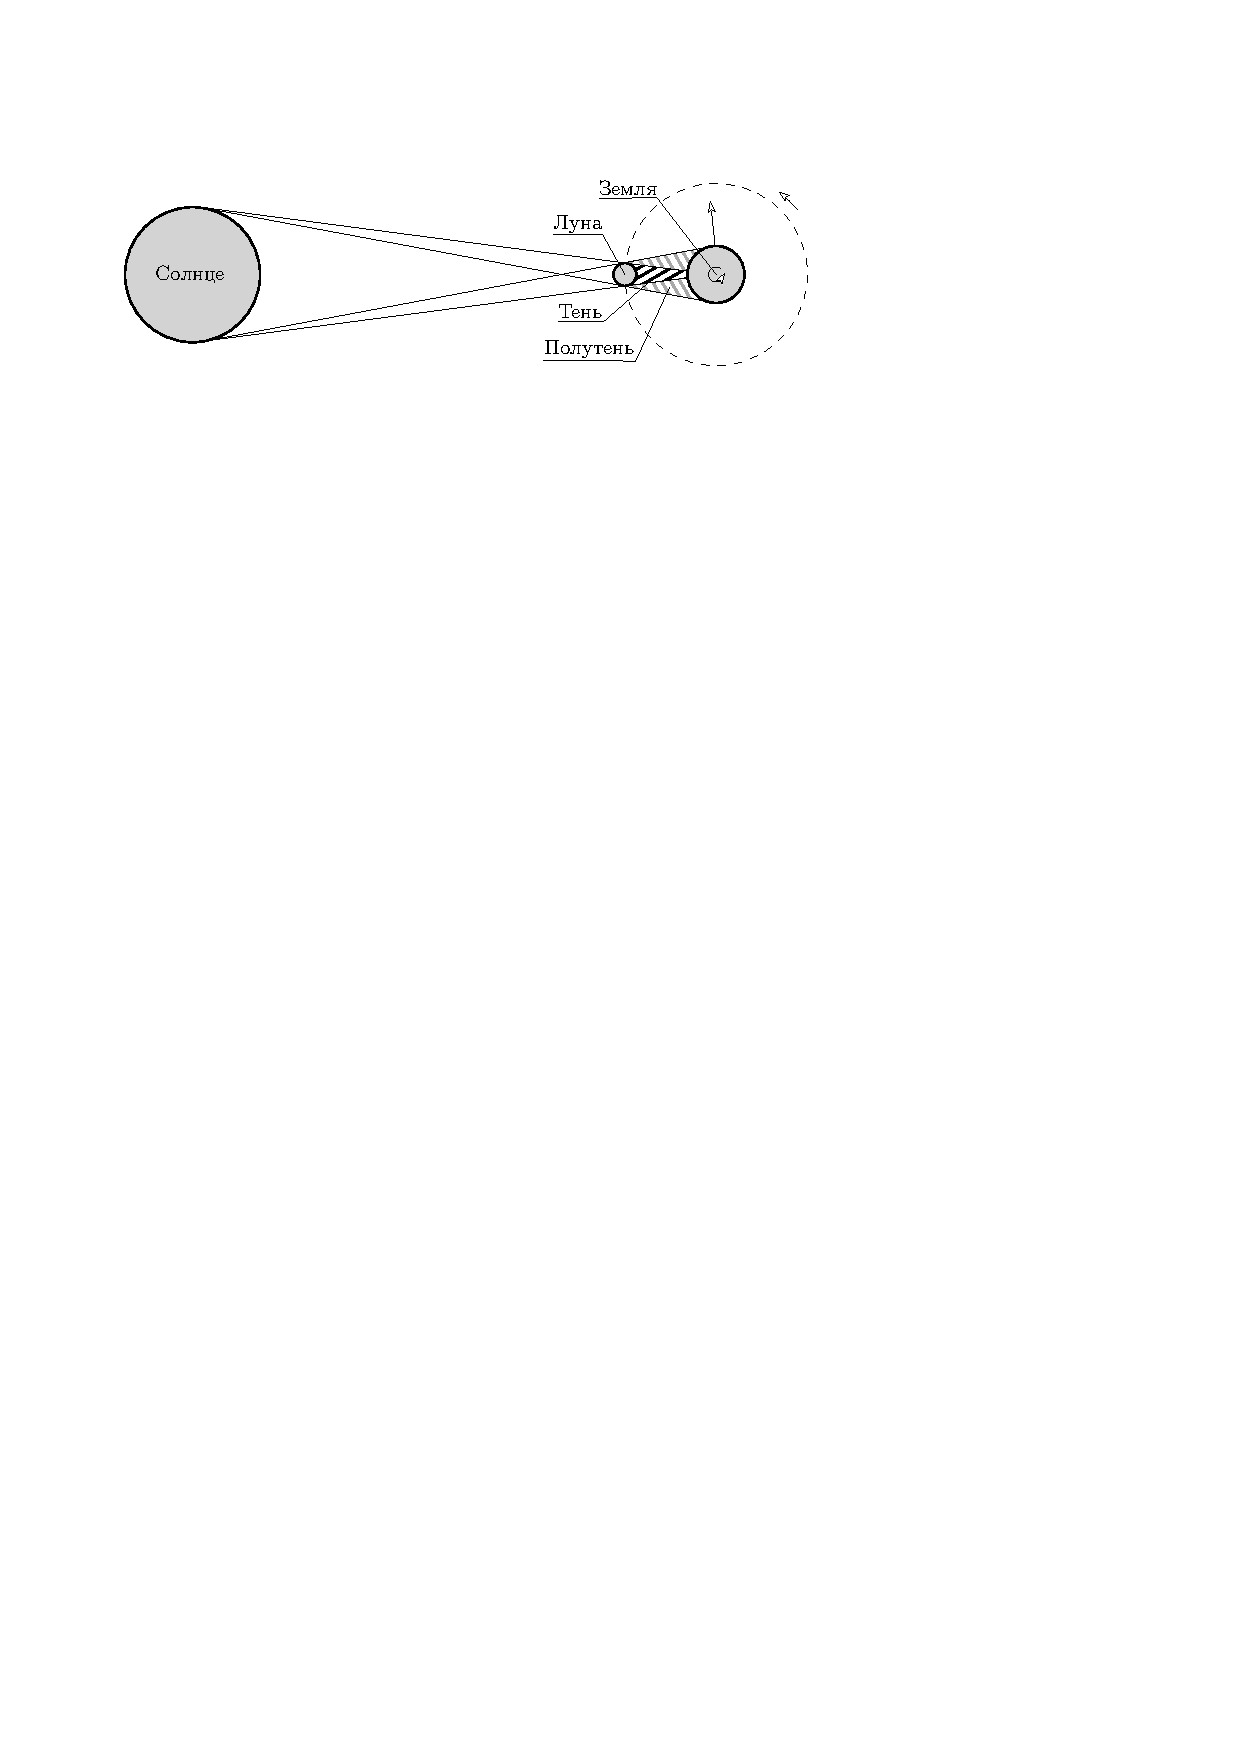
\includegraphics[width = 1.05\textwidth]{full_eclipse}
\caption{Полное солнечное затмение}
\end{figure}

\subsubsection{Кольцеобразное солнечное затмение}
При кольцеобразном солнечном затмении Луна относительно Земли расположена так, 
что конус её тени не достаёт до поверхности планеты, и вокруг Луны можно 
наблюдать яркое кольцо незакрытой части солнечного диска (Рис.9).
\begin{center}
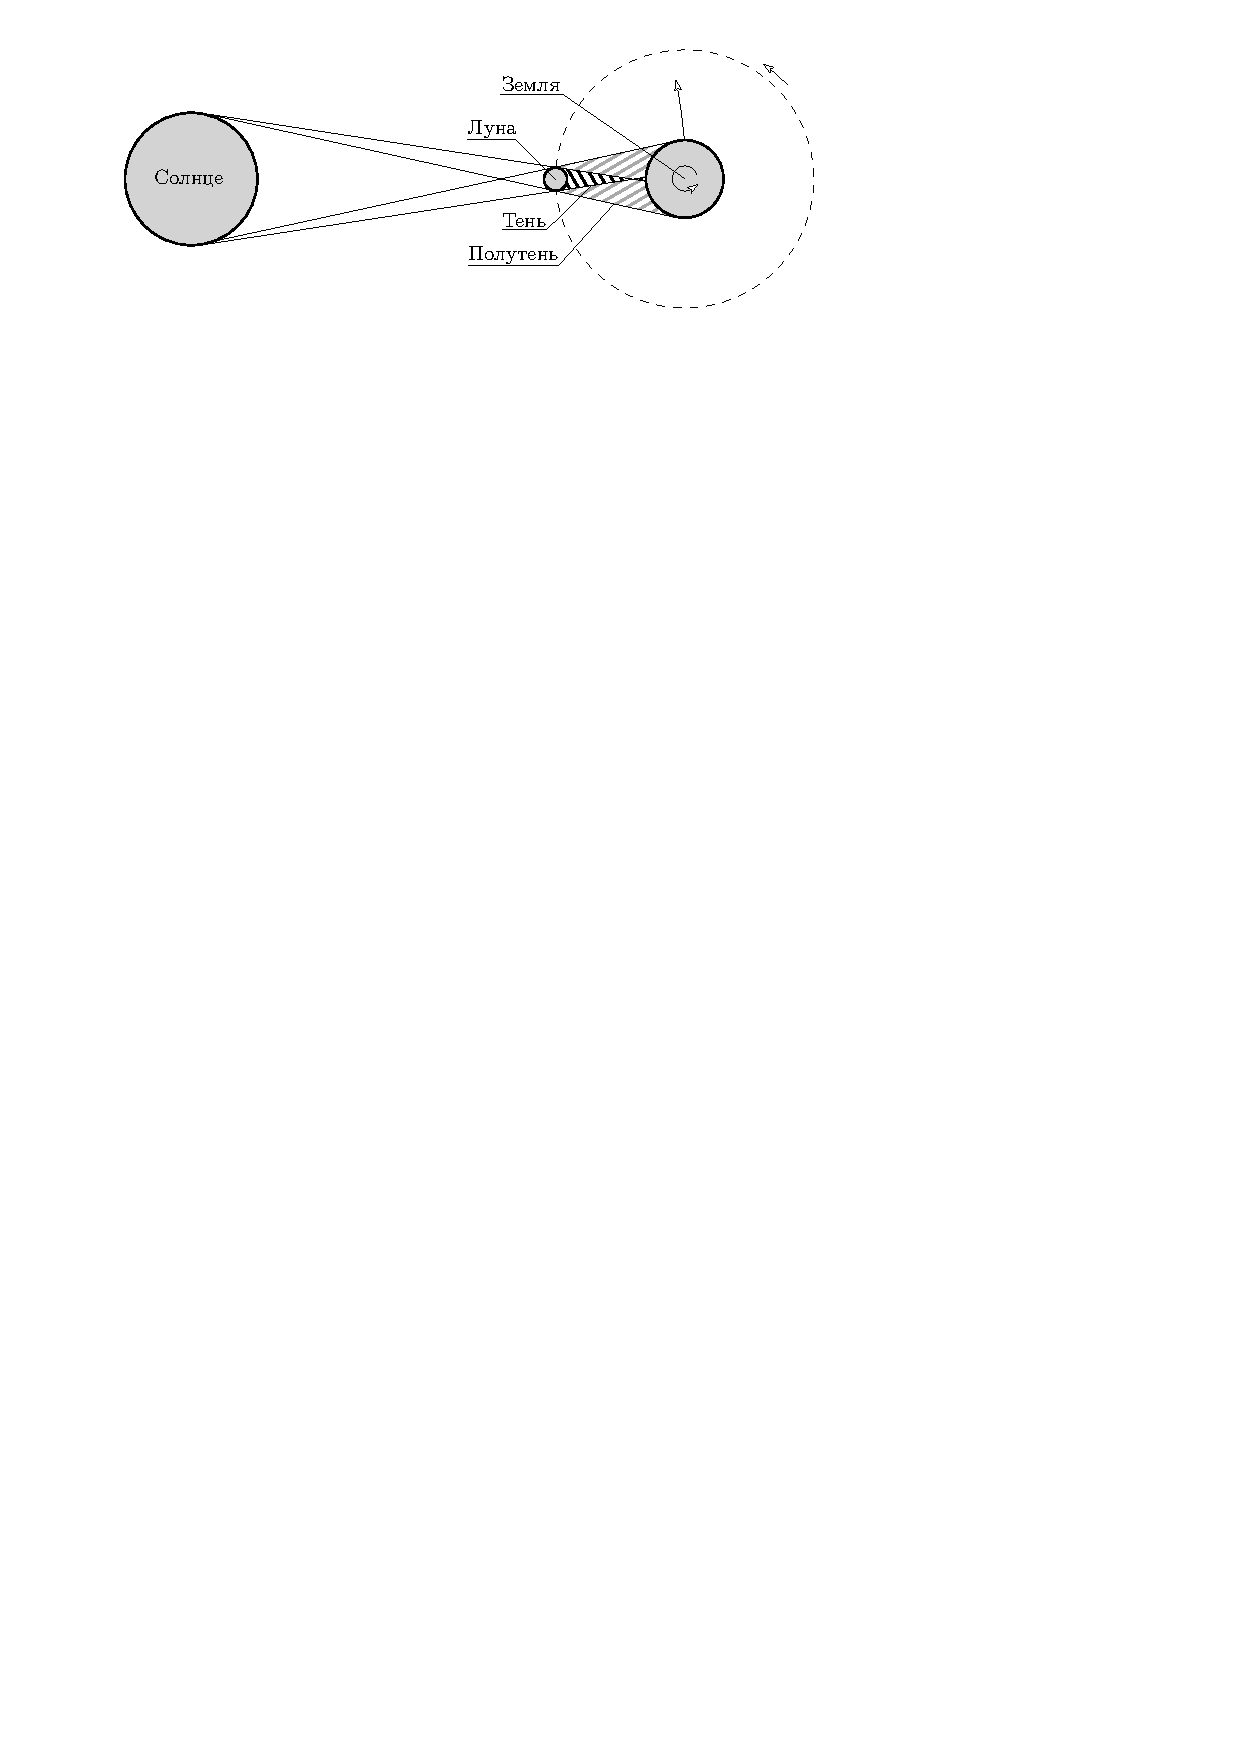
\includegraphics[width = 0.95\textwidth]{partly-eclipse}
\begin{figure}[h!]
\caption{Кольцеобразное солнечное затмение}
\end{figure}
\end{center}
\subsubsection{Лунное затмение}

Лунное затмение в отличие от солнечного, видно со всего ночного полушария. 
Диаметр земной тени на расстоянии Луны превышает размер последней примерно в 
2.5-3 раза (Рис.10).

\textbf{Сарос} --- промежуток  времени, по прошествии которого солнечные и 
лунные затмения повторяются в прежнем порядке.

Этот период почти в точности равен:
\begin{enumerate}
\item 242 драконических месяца;
\item 223 синодических месяца;
\end{enumerate}

Таким образом, сарос длится примерно 18 лет 11 дней 8 часов.

\textbf{Синодический месяц} --- промежуток времени между одинаковыми фазами 
Луны. Он равен 29.53 суток.

\textbf{Драконический месяц} --- промежуток времени между двумя 
последовательными прохождениями Луны через один и тот же узел орбиты. 
Драконический месяц равен 27.21 суток.
\begin{center}
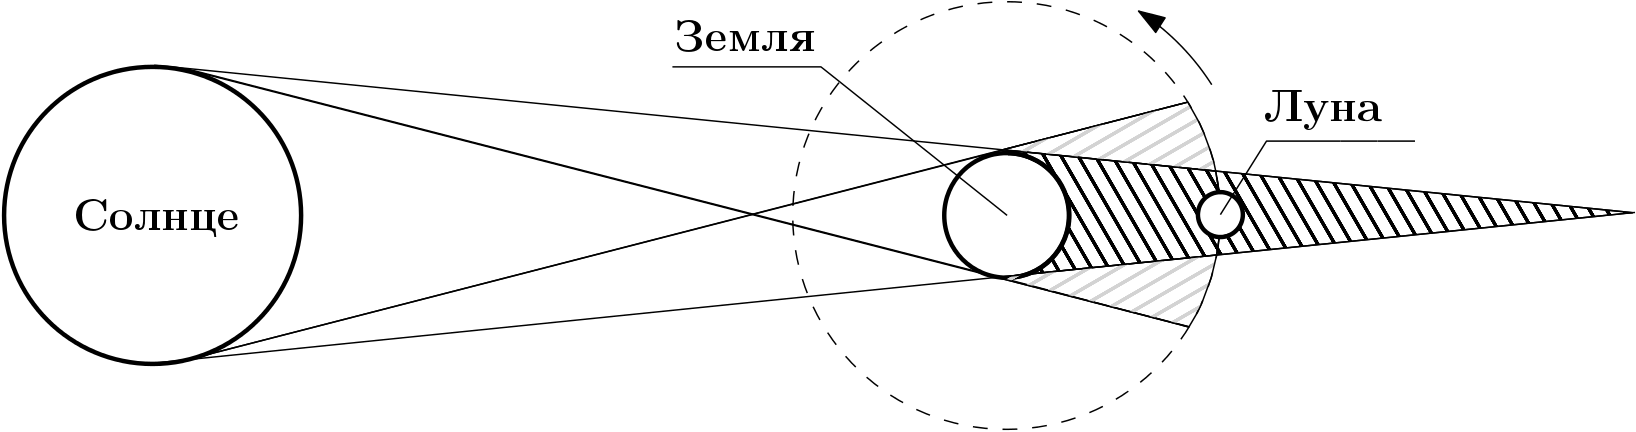
\includegraphics[scale=0.27]{moon-eclipse}
\begin{figure}[h!]
\caption{Лунное затмение}
\end{figure}
\end{center}
\subsubsection{Фаза затмения}
Очень важной характеристикой любого затмения является его фаза. \textbf{Фаза 
затмения} --- отношение закрытой части диаметра затмеваемого тела, проходящей 
через уентр затмевающего тела, к полному диаметру затмеваемого тела. Для 
полного затмения эта величина считается немного иначе (см. ниже). Для Луны 
затмевающим "телом" является тень Земли. Фазу частного и полного затмения можно 
вычислить по слейдующим формулам (Рис.11):
\begin{equation}\Phi_{\text{ч}}=\frac{x}{D}
\end{equation} \text{ и } \begin{equation}\Phi_{\text{п}}=1+\frac{d}{D}
\end{equation}
Где $D$ --- диаметр затмеваемого тела.
\begin{center}
\includegraphics[width = 0.3\textwidth]{phases}
\includegraphics[width = 0.3\textwidth]{phases-2}
\begin{figure}[h!]
\caption{Частное и полное затмение}
\end{figure}
\end{center}

Иногда вводят такое понятие, как \textbf{площадная фаза затмения}, т.е. 
отношение площади закрытой части диска затмеваемого диска к полоной площади его 
диска. Чаще площадную фазу используют применительно к двойным звёздам, когда 
считают падение блеска при затмении одной звезды другой.

%\subsection{Прецессия}

Ось вращения Земли совершает прецессионное движение --- описывает вокруг оси эклиптики  конус радиусом основания 23.5$^\circ$ с периодом около 26 000 лет. Из-за этого меняется положение полюс мира. Например, сейчас полюс мира практически совпадает с Полярной звездой ($\alpha$ Малой Медведицы), а 15 000 лет назад роль Полярной звезды играла Вега ($\alpha$ Лиры). Если считать, что величина прецессии постоянна, то полюсы мира описывают вокруг полюсов эклиптики малые круги с радиусом 23.5$^\circ$. В действительности же величина прецессии меняется, поэтому путь полюсов мира представляет собой не окружность, а спираль.

Поворот оси Земли имеет различные последствия. Во-первых, меняется продолжительность тропического года, он становится примерно на 20 минут короче звёздного. Во-вторых, из-за прецессии меняется вид звёздного неба, хотя происходит это очень медленно (Рис.12).
\begin{center}
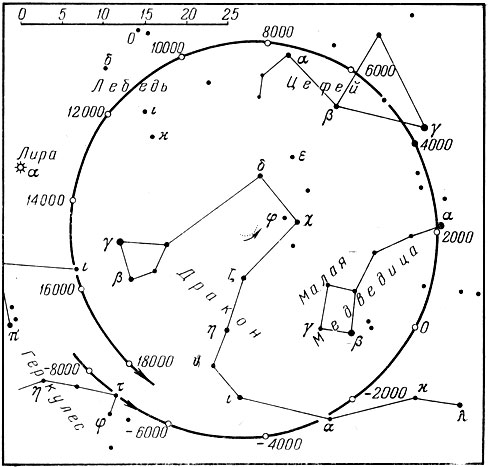
\includegraphics[scale=0.46]{Precess}
\begin{figure}[h!]
\caption{Прецессионное движение северного полюса мира}
\end{figure}
\end{center}
%\subsection{Точки Лагранжа}

{\itshape Точками Лагранжа} --- точки, в вращающейся системе из двух
массивных тел, в которых третье тело с пренебрежимо 
малой массой, не испытывающее воздействие никаких 
других сил, кроме гравитационных, со стороны двух 
первых тел, может оставаться неподвижным относительно 
этих тел (Рис.\ref{pic:lagr-points}). В этих точках гравитационные силы, действующие на малое тело, уравновешиваются центробежной силой.

Точки $L_1$, $L_2$ и $L_3$ лежат на одной прямой, 
соединяющей два массивных тела. Точки $L_4$ и $L_5$ 
образуют равносторнние треугольники с массивными 
телами.

Для расстояний до точек $L_1$, $L_2$ и $L_3$ от 
центра масс справедливы следующие выражения:
\begin{equation}r_1=R\left(1-\sqrt[3]{\frac{\alpha}
{3}}\right) \quad r_2=R\left(1+\sqrt[3]{\frac{\alpha}
{3}}\right) \quad r_3=\left(1+\frac{5}{12}\alpha\right)
\end{equation}
где $\alpha=M_1/(M_2+M_3)$, $R$ --- расстояние между 
телами, $M_1$ --- масса более массивного тела, $M_2$
 --- масса второго тела.

Если $M_2\ll M_1$, то точки $L_1$ и $L_2$ находятся 
примерно на равном расстоянии от тела $M_2$. 
Примерное значение этого расстояния можно получить
из соотношения
\begin{equation}r\approx R\sqrt[3]{\frac{M_2}{3M_1}}
\end{equation}
\begin{center}
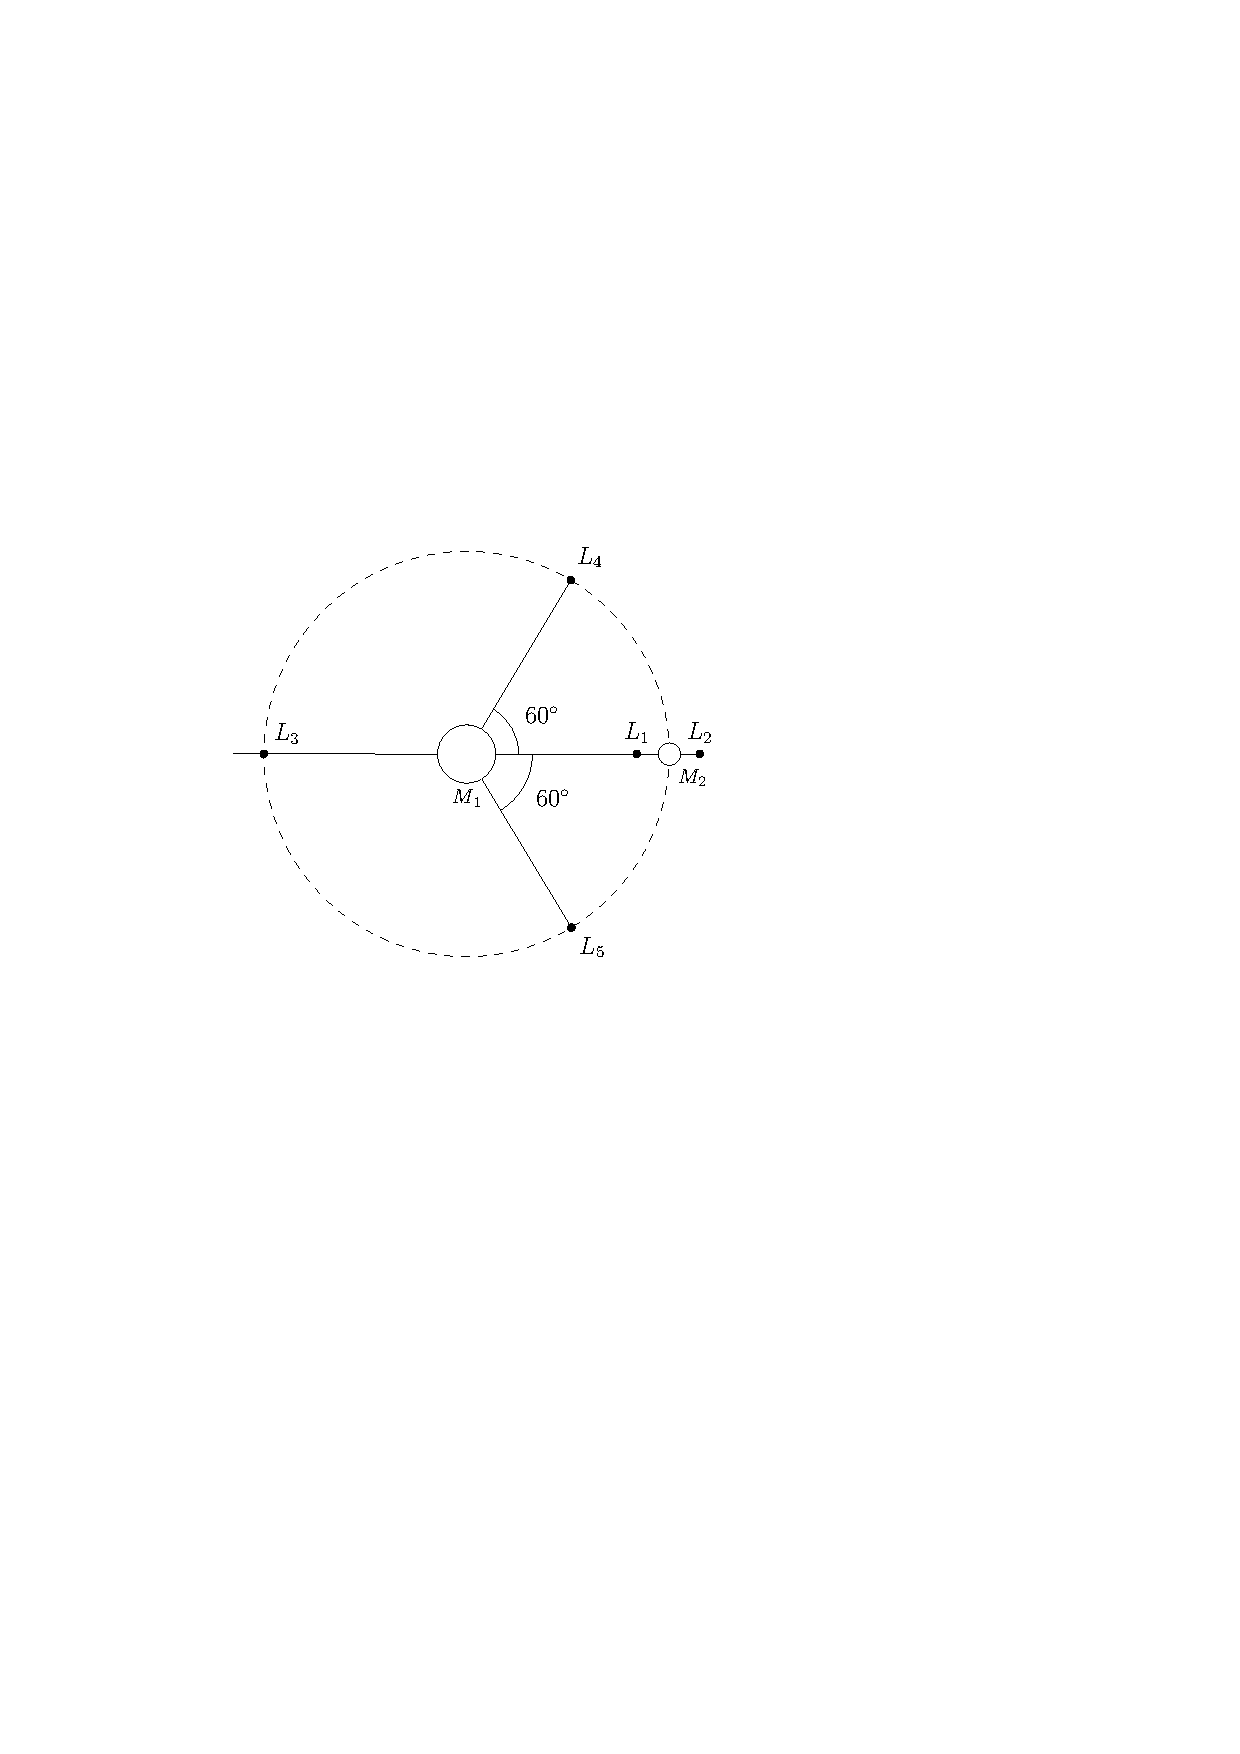
\includegraphics[width = 0.5\textwidth]{lagr-points}
\begin{figure}[h!]
\caption{Точки Лагранжа}\label{pic:lagr-points}
\end{figure}
\end{center}
%\subsection{Расстояние и размеры}
\textit{Годичный параллакс} --- это угол, под которым видно орбиту Земли с какой-либо звезды.
\begin{equation}r=\frac{1}{\pi}
\end{equation}
Где $r$ --- расстояние до звезды (в парсеках), $\pi$ --- годичный параллакс звезды (в секундах).
\begin{figure}[!h]
\centering
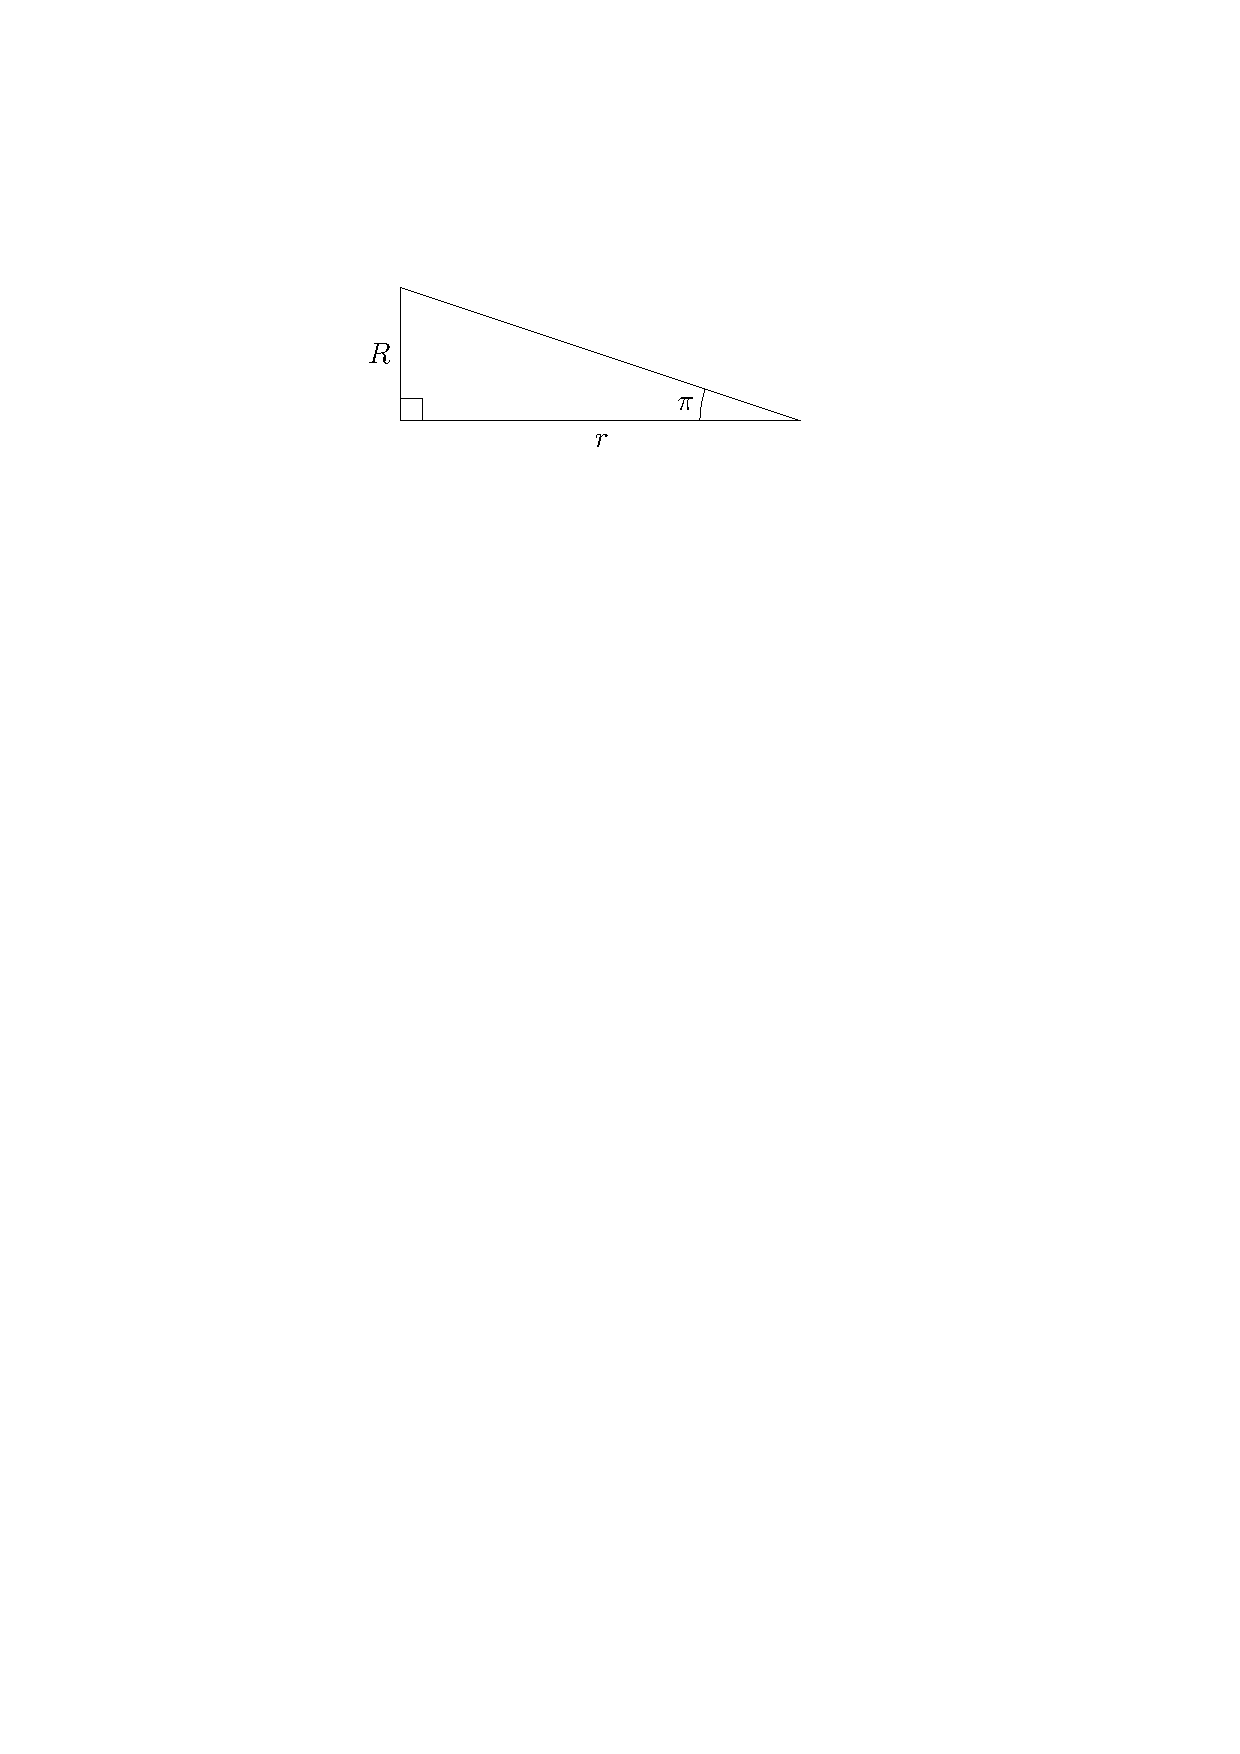
\includegraphics[width = 0.37\textwidth]{1-second}
\caption{Параллакс в одну секунду}
\end{figure}

Если $R$ --- радиус орбиты Земли, $r$ --- расстояние до объекта, $\pi$ --- годовой параллакс, то параллакс будет равен $\pi=1''$ с расстояния $r=1$пк.

В общем случае: 
\begin{equation}
\sin\pi=R/r
\end{equation}

Где $R$ и $r$ имеют одинаковые еденицы измернеий, но так как в одном парсеке 206265 а.е. и в одном радиане 206265 секунд, то,записывая радиус орбиты Земли в а.е., а расстояние звезды в парсеках, параллакс получается в секундах. Также, можно изменить $\sin\pi$ на $\pi$, потому что угол $\pi$ является малым углом. Таким образом, получается следующая формула:\begin{equation}
r_{\text{пк}}=\frac{1\text{ а.е.}}{\pi_{\text{сек}}}
\end{equation}


\textit{Горизонтальный параллакс} --- это угол, под которым видно радиус Земли, при положении светила на горизонте.
\begin{equation}r=\frac{R_{\text{З}}}{\sin p_0}=\frac{3438'}{p_0'}R_{\text{З}}=\frac{206265''}{p_0''}R_{\text{З}}
\end{equation}
Где $R_{\text{З}}$ --- радиус Земли, $p_0$ --- горизонтальный экваториальный параллакс.

\textbf{Правило Тициуса-Боде} --- эмпирическая формула приблизительно описывающая радиусы орбит планет от Солнца:
\begin{equation}r=\frac{3\cdot 2^n+4}{10}
\end{equation}
Где $n=-\infty, 0, 1, 2...$

\textit{Угловой размер объекта} --- это угол, под которым видно радиус объекта с Земли.
\begin{equation}\rho=\frac{R}{r}
\end{equation}
Где $R$ --- радиус объекта, $\rho$ --- угловые размеры объекта, $r$ --- растояние до объекта. Здесь также можно использовать приближение для малых углов: $\sin\rho\approx\rho$

%\section{Конические сечения}
\subsection{Эллипс}
{\bfseries \term{Эллипс}} --- плоская замкнутая кривая, сумма 
расстояний от любой точки которой до двух фиксированных 
точек, называемых фокусами, постоянна и равна 
удвоенной большой полуоси эллипса.
\begin{equation}|F_1 M|+|F_2M|=const=2a
\end{equation}

Главные отрезки эллипса: \term{большая полуось} 
($a$), \term{малая полуось} ($b$), \term{ 
фокусное расстояние} ($c$). Они связаны следующим 
соотношением: $b^2+c^2=a^2$, что несложно вывести из 
определения эллипса.

\term{Эксцентриситет} ($e$) --- числовая 
характеристика, показывающая степень отклонения от 
окружности. Для эллипса $e$ лежит в интервале $(0, \, 1)$ и
определяется следующей формулой:\begin{equation}
p=\frac{b^2}{a}=a(1-e^2)=b\sqrt{1-e^2}
\end{equation}

\begin{figure}[h!]
\centering
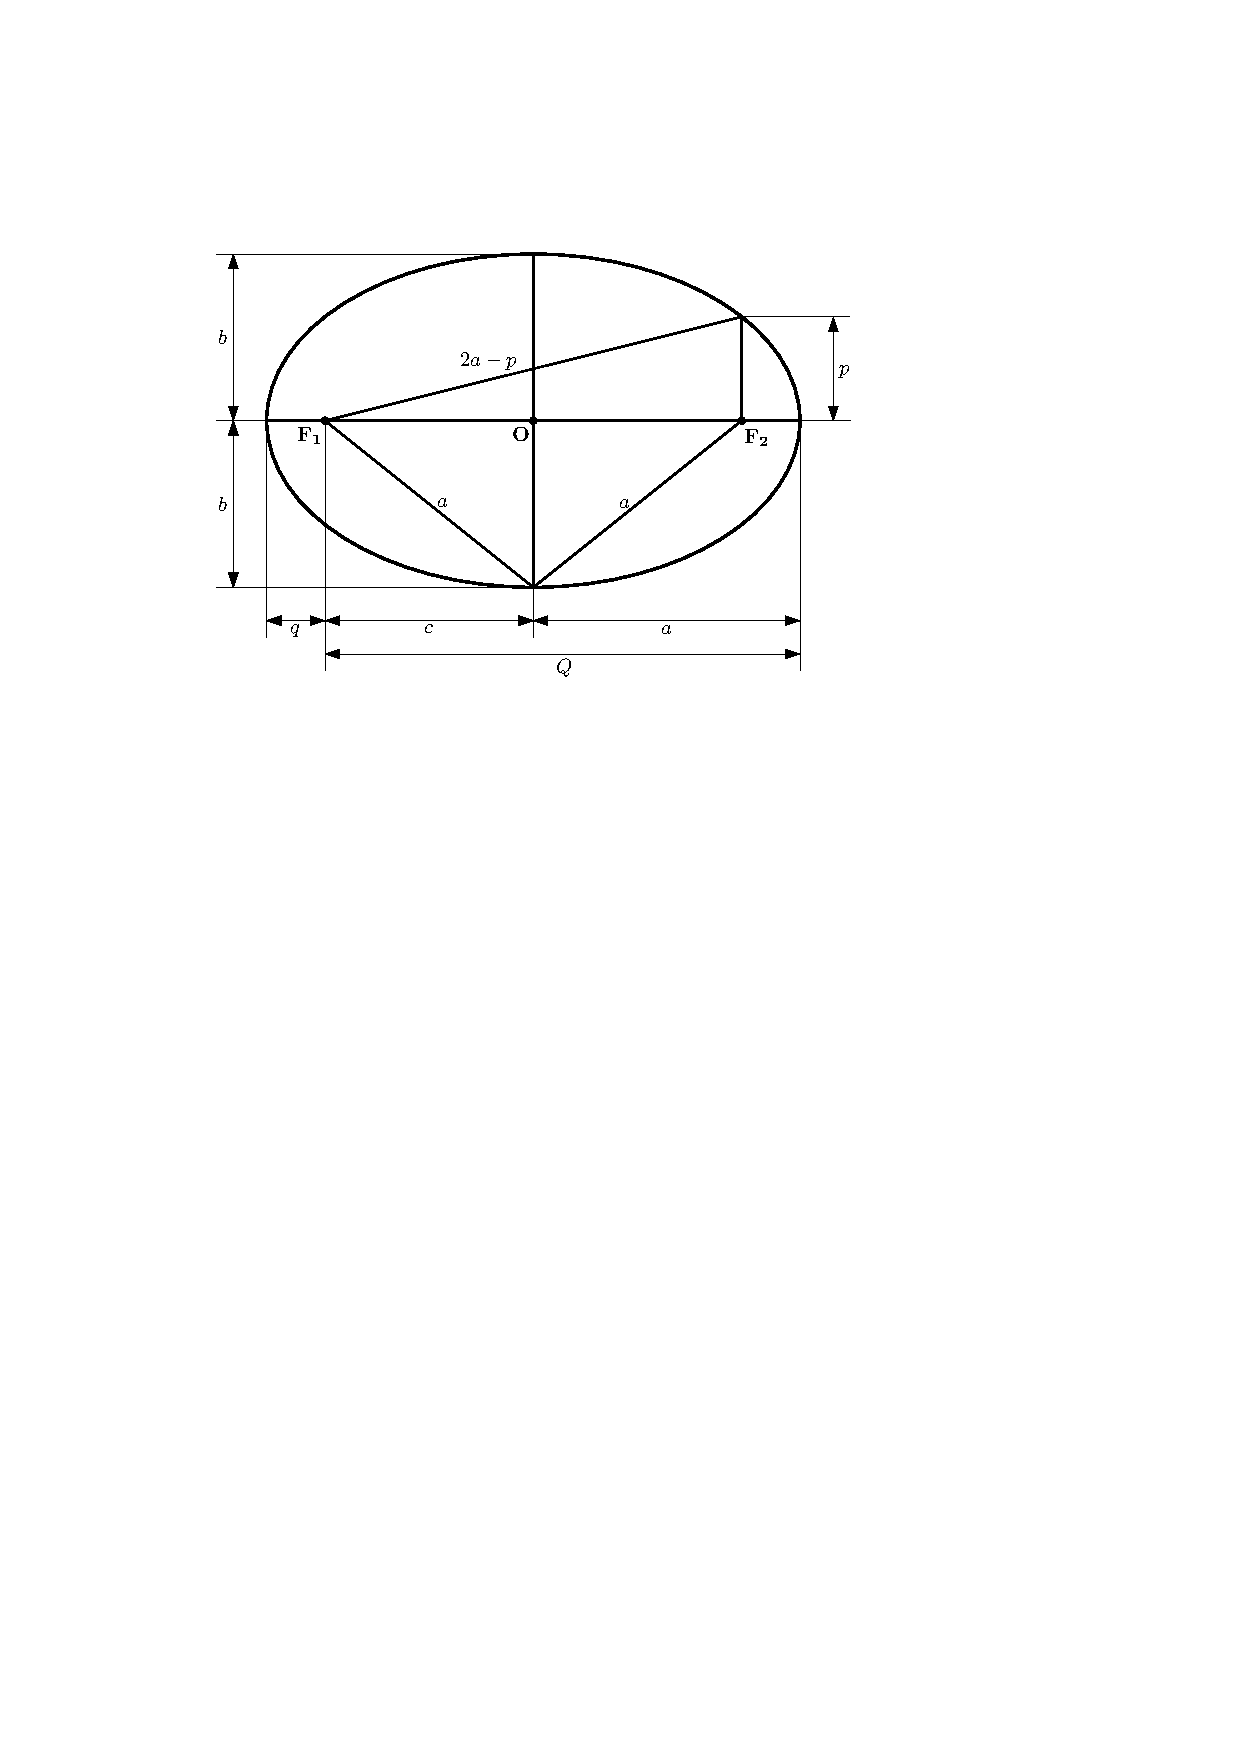
\includegraphics[width = 0.8\textwidth]{Ellips}
\caption{Эллипс}
\end{figure}

\term{Апоцентр} --- наиболее удаленная точка
от заданного фокуса точка эллипса. Из определения эллипса
вытекает соотношение для расстояния от фокуса до 
апоцентра ($Q$):\begin{equation}
Q = a (1 + e)
\end{equation}

\term{Перицентр} --- ближайшая точка
точка эллипса к заданному фокусу . Из определения эллипса
вытекает соотношение для расстояния от фокуса до 
перицетра ($q$):\begin{equation}
q = a (1 - e)
\end{equation}

\term{Фокальный параметр} ($p$) --- длина перпендикуляра,
проведенного из фокуса до точки пересечения с эллипсом.
Из теоремы Пифагора и определения эллипса следует 
нижеприведенная формула для расчета его длины. 
\begin{equation}
p = a(1 - e^2)
\end{equation}

\term{Площадь эллипса} ($S$) --- площадь части 
плоскости, ограниченной эллипсом. Выражение для площади 
эллипса можно находить интегрированием по полярному углу, 
используя уравнение эллипса в полярных координатах или 
пользуясь свойством аффинного преобразования сжатия из 
выражения площади окружности с радиусом $a$:
\begin{equation}
S=\pi ab
\end{equation}

%Радиус кривизны дуги эллипса в зависимости от расстояния 
%$x$ от фокуса:
%\begin{equation}
%R=\frac{(2ax-x^2)^{3/2}}{ab}
%\end{equation}
%\begin{center}
%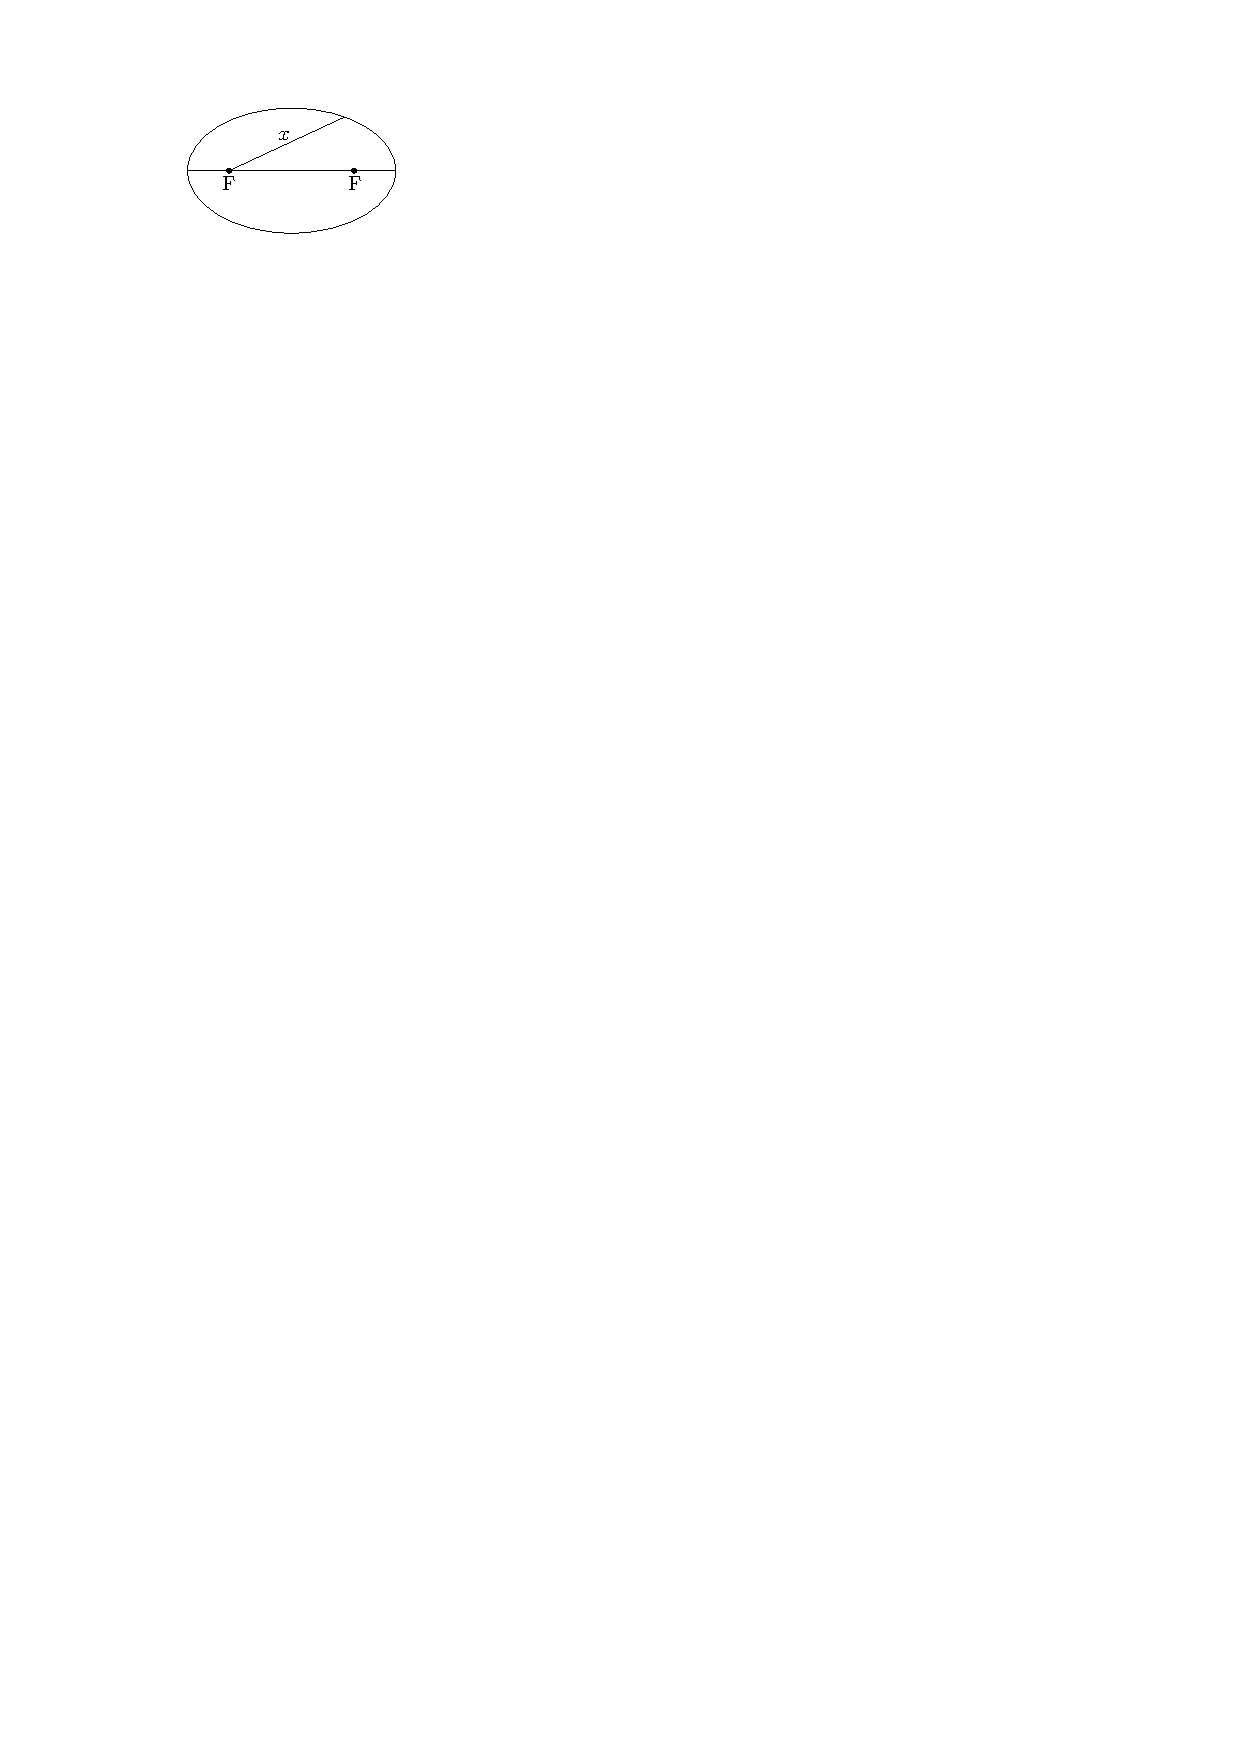
\includegraphics[width = 0.3\textwidth]{rad-curv}
%\begin{figure}[!h]
%\caption{К вычислению радиуса кривизны эллипса}
%\end{figure}
%\end{center}

{\itshape Уравнение эллипса} в декартовых координатах 
представляет собой уравнение замкнутой кривой второго 
порядка, канонический вид которого имеет следующий вид:
\begin{equation}
\frac{x^2}{a^2}+\frac{y^2}{b^2}=1
\end{equation}

Его можно представить параметрическом виде:\begin{equation}
\left\{\begin{aligned}[lcl]
&x=a\cos t;\\
&y=b\sin t,\\
\end{aligned}
\right.
\end{equation}
где параметр $t \in [0, \, 2\pi)$.

В полярных координатах уравнение принимает следующий вид:
\begin{equation}
r=\frac{p}{1\pm e\cos\phi},
\end{equation} 
где $\varphi$ --- \term{истинная аномалия} --- угол 
{\slshape перицентр -- фокус -- заданная точка}, 
отсчитываемый в сторону движения по эллипсу. При 
положительном знаке перед $e$ второй фокус эллипса будет 
находится в точке $(0, \, 2c)$, а при отрицательном --- в 
точке $(\pi, \, 2c)$.\\

Кроме этого, эллипс обладает важным {\itshape оптическим 
свойством}, которе можно сформулировать так: свет от источника в одном из фокусов, 
	отражается эллипсом так, что отражённые лучи пересекаются 
	во втором фокусе или, что тоже самое, касательная к эллипсу в заданной точке образует с фокальными радиусами в данной точке равные острые углы.






 

\subsection{Парабола}

\begin{wrapfigure}[8]{r}{0.45\tw}
    \centering
    \vspace{-0.7pc}
    \tikzsetnextfilename{parabola}
    \begin{tikzpicture}
       \def\xmax{2.4}
       \def\k{0.33}
       \def\x{1/(4*\k)}


       \tkzDefPoint(-\xmax,{\xmax*\xmax*\k}){X0}
       \foreach \x in {-2.4,-2.35,...,2.4} {
           \def\y{\x*\x*\k}
           \tkzDefPoint(\x,\y){X1}
           \tkzDrawSegment[thick](X0,X1)
           \tkzDefShiftPoint[X1](0,0){X0}
       }

       \tkzDefPoint(0,0){O}
       \tkzDefPoint(0,{1/(4 *\k)}){F}
       \tkzDefPointBy[homothety=center O ratio -1](F) \tkzGetPoint{D}
       \tkzDefPointBy[homothety=center O ratio 2](F) \tkzGetPoint{F'}
       \tkzDefPointWith[orthogonal,K={2*\k *\xmax}](D,F) \tkzGetPoint{D1}
       \tkzDefPointBy[homothety=center D ratio -1](D1) \tkzGetPoint{D2}

       \tkzDefPointWith[orthogonal,K=-1](F,D) \tkzGetPoint{P}
       \tkzDefPointBy[projection = onto D1--D2](P)  \tkzGetPoint{P'}

       \tkzDefPoint(-\x, \k*\x*\x){X}
       \tkzDefPointBy[projection = onto D1--D2](X)  \tkzGetPoint{X'}

       \tkzMarkRightAngles[size=0.2](D2,D,F F',F,P D,P',P D2,X',X)


       \tkzDrawSegments[semithick](D1,D2 F,P P,P' F,X X,X')

       \tkzDrawSegment[dim={{$q$},{\xmax*0.9},right=1mm, midway}](F,O)
       \tkzDrawSegment[dim={{$q$},{\xmax*0.9},right=1mm, midway}](O,D)

       \tkzLabelPoint[above right=-1pt](F){$\mathbf{F}$}
       \tkzLabelPoint[below right=-2pt](O){$\mathbf{O}$}
       \tkzLabelPoint[below left=-2pt](X){$\mathbf{X}$}
       \tkzLabelSegment[above](F,P){$p$}
       \tkzLabelSegment[left](P,P'){$p$}
       \tkzLabelSegment[above left=-4pt](F,X){$r$}
       \tkzLabelSegment[right](X,X'){$d$}

       \tkzDrawSegments[dash dot, semithick](D,F')
       \tkzDrawSegments[semithick](D,F)

       \tkzDrawPoints(O, F, P, X)
        
    \end{tikzpicture}
    \caption{Парабола}
    \label{pic:parabola}
\end{wrapfigure}
\term{Парабола}~--- геометрическое место точек, равноудалённых от заданной прямой~--- \term{директрисы} параболы, и заданной точки~--- \term{фокуса} параболы.

Получим из определения параболы её уравнение в декартовых координатах. Пусть расстояние между фокусом и директрисой параболы равно $p$. Из определения ясно, что существует точка параболы $P$, располагающаяся в середине перпендикуляра, опущенного из фокуса на директрису. Расположим параболу так, чтобы эта точка оказалась в начале координат, директриса задавалась уравнением $x = -p/2$, а фокус имел координаты $(p/2, 0)$.

Приравняем расстояния от произвольной точки параболы с координатами $(x, y)$ до директрисы и до фокуса:
\begin{gather*}
    x + \frac{p}{2} = \sqrt{\left(x - \frac{p}{2} \right)^2 + y^2},\\
    x^2 + \frac{p^2}{4} + px = x^2 + \frac{p^2}{4} - px + y^2,\\
    y^2 = 2px. \tag{\theequation}
\end{gather*}

Полученное равенство является каноническим уравнением параболы в декартовых координатах. В силу симметрии данного уравнения, перпендикуляр, опущенный из фокуса на директрису, является \imp{осью} параболы, а точка $P$~--- её \imp{вершиной}.

Легко заметить, что длина перпендикуляра, опущенного из фокуса на параболу, равна $p$. Этот отрезок называется \term{фокальным параметром}, а его длина, как следует из вышесказанного, равна расстоянию от фокуса до директрисы.

\begin{wrapfigure}[9]{r}{0.4\tw}
    \centering
    \vspace{-1pc}
    \tikzsetnextfilename{parabola-polar-coord}
    \begin{tikzpicture}[scale=1.2]
        \footnotesize
        \clip (-.3, -0.7) rectangle + (3.5, 3.2);

        \coordinate (xy) at (1, 1.11) {};
        \coordinate (F) at (.3, 0) {};

        \draw [line width = .7pt](3, 2) .. controls (-1, .5) and (-1, -.5) .. (3, -2);

        \draw [-latex] (.3, -2.2) -- (.3, 2.5);
        \draw [-latex] (-1, 0) -- (3.2, 0);

        \draw (F) circle (.5);
        \draw (F) circle (1);
        \draw (F) circle (1.5);
        \draw (F) circle (2);
        \draw (1.61, 0) [-latex, line width=1pt] arc (0:57.8:1.31);
        \draw [-latex, line width=1pt] (.3, 0) -- (1, 1.11);

        \draw (1.05, 1.05) node [anchor=south east] {\tiny{$(x', y')$}};
        \draw (F) node [anchor=north west] {$F$};
        \draw (.65, .55) node [anchor=west] {$\vec r$};
        \draw (1.5, .7) node [anchor=north east] {$\boldsymbol{\varphi}$};
        \draw (3.2, 0) node [anchor=north east] {$x'$};
        \draw (-.1, 2.5) node [anchor=north west] {$y'$};

        \draw (F) [fill=white] circle(.025);
        \draw (xy) [fill=white] circle(.025);
    \end{tikzpicture}
    \caption{}
    \label{pic:parabola-polar-coord}
\end{wrapfigure}
Перенесем теперь фокус параболы в начало координат и получим уравнение параболы в полярных координатах. Для этого нужно сделать такую замену: $x' \hookrightarrow x - p/2$, значит $x \hookrightarrow x' + p/2$, а $y' \hookrightarrow y$. Запишем уравнение параболы в новых координатах:
\begin{gather*}
    y^2 = 2px,\\
    (y')^2 = 2 p \left(x' + \frac{p}{2} \right).
\end{gather*}
Перейдём в полярные координаты в полученном равенстве:
\begin{gather*}
    r^2 \sin^2 \varphi = p^2 + 2pr\cos \varphi,\\
    r^2 \cdot \sin^2 \varphi - r \cdot 2 p  \cos \varphi - p^2,\\
    D = 4p^2 \cos^2 \varphi + 4 p^2 \sin^2 \varphi = 4 p^2,\\
    r = \frac{2p \cos \varphi \pm 2p}{2\sin^2 \varphi}, \quad r \geqslant 0,\\
    r = \frac{p (\cos \varphi + 1)}{1 - \cos^2 \varphi} = \frac{p (\cos \varphi + 1)}{(1 - \cos\varphi)(1 + \cos\varphi)} = \frac{p}{1 - \cos \varphi}.
\end{gather*}
Если же параболу развернуть на $180^\circ$, в знаменателе будет знак плюс. Это завершает вывод уравнения параболы в полярных координатах:
\begin{equation}
    r = \frac{p}{1 \pm \cos \varphi}.
\end{equation}

\begin{wrapfigure}{r}{0.45\tw}
    \centering
    \vspace{-.5pc}
    \tikzsetnextfilename{parabola-optic-property}
    \begin{tikzpicture}[scale=1.2]
        \footnotesize
        \clip (-.4, -1) rectangle + (4, 3.5);

        \coordinate (xy) at (1, 1.11) {};
        \coordinate (F) at (.3, 0) {};

        \draw [line width = .7pt](3, 2) .. controls (-1, .5) and (-1, -.5) .. (3, -2);

        \draw [-latex] (0, -2.2) -- (0, 2.5);
        \draw [-latex] (-1, 0) -- (3.5, 0);

        \draw [-latex, line width=1pt] (F) -- (xy);
        \draw [-latex, line width=1pt] (xy) -- (2, 1.11);
        \draw [-latex, line width=1pt] (xy) -- (2, 1.67);
        \draw (xy) -- (3, 1.11);
        \draw [dashes] (3, 2.21) -- (-.5, 0.29);

        \draw (1.2, 1.11) node [anchor=south east] {$(x, y)$};
        \draw (F) node [anchor=north] {$F$};
        \draw (.65, .55) node [anchor=west] {$\vec r$};
        \draw (1.5, 1.11) node [anchor=north] {$\vec x$};
        \draw (1.5, 1.39) node [anchor=south] {$\vec t$};

        \draw (3.5, 0) node [anchor=north east] {$x$};
        \draw (0, 2.5) node [anchor=north west] {$y$};

        \draw (F) [fill=white] circle(.025);
        \draw (xy) [fill=white] circle(.025);
    \end{tikzpicture}
    \caption{}
    \label{pic:parabola-optic-property}
\end{wrapfigure}
Как и все конические сечения, парабола обладает \imp{оптическим свойством}, которое формулируется таким образом: пучок лучей, параллельных оси параболы, отражаясь в последней, собирается в её фокусе. И наоборот, свет от точечного источника, находящегося в фокусе, отражается параболой в пучок параллельных её оси лучей.

Аналогично доказательству оптического свойства эллипса рассмотрим случай только верхней ветви. Выберем на ней произвольную точку $(x, y)$. Тогда вектор, определяющий направление луча из фокуса в выбранную точку задается вектором $\vec r = (x - p/2, y)$. Направление, соответствующее оси параболы, зададим единичным вектором $\vec x = (1, 0)$, так как ось параболы с каноническим уравнением совпадает с осью абсцисс. Остается найти вектор $\vec t$ касательной в точке $(x, y)$. Для верхней ветви параболы каноническое уравнение эквивалентно $y = \sqrt{2px}$. Найдем производную данной функции:
\begin{gather*}
    y' = \frac{2p}{2\sqrt{2px}} = \sqrt{\frac{p}{2x}}.
\end{gather*}
Значит направляющий вектор касательной можно представить в виде
\begin{equation*}
    \vec t =
    \begin{pmatrix}
        1\\
        y'_x
    \end{pmatrix} =
    \begin{pmatrix}
        1\\
        \sqrt{\dfrac{p}{2x}}
    \end{pmatrix}.
\end{equation*}

Остается проверить равенство косинусов углов между векторами $\vec r$ и $\vec t$ и векторами $\vec x$ и $\vec t$:
\begin{gather*}
    \frac{\scalar{r}{t}}{|\vec r| | \vec t|} = \frac{\scalar{x}{t}}{|\vec x| |\vec t|},\\
    \scalar{r}{t} = |\vec r| \scalar{x}{t},\\
    \left(x - \frac{p}{2}\right)\cdot 1 + y \cdot \sqrt{\frac{p}{2x}}  = \sqrt{\left( x - \frac{p}{2} \right)^2 + y^2 } \left(1 \cdot 1 + 0 \cdot \sqrt{\frac{p}{2x}} \,\right),\\
    \left(x - \frac{p}{2}\right)^2 + \frac{y^2 p}{2x} + 2 y \sqrt{\frac{p}{2x}} \left(x - \frac{p}{2}\right) = \left(x - \frac{p}{2}\right)^2 + y^2,\\
    2  \sqrt{\frac{p}{2x}} \left(x - \frac{p}{2}\right) =  y \left( 1 - \frac{p}{2x} \right),\\
    \sqrt{\frac{4x^2p}{2x}} \left(1 - \frac{p}{2x}\right) =  y \left( 1 - \frac{p}{2x} \right),\\
    \sqrt{2xp}  =  y.
\end{gather*}
Получено уравнение верхней ветви параболы, которому, очевидно, координаты точки, принадлежащей параболе, удовлетворяют. Следовательно, оптическое свойство доказано.

Покажем, что парабола является коническим сечением. Для этого рассмотрим каноническое уравнение конической поверхности
\begin{equation*}
    \frac{x^2}{a^2} + \frac{y^2}{b^2} - \frac{z^2}{c^2} = 0
\end{equation*}
и секущую плоскость, параллельную образующей конуса и задаваемую уравнением
\begin{equation*}
    z = \frac{c(x + d)}{a},
\end{equation*}
где коэффициенты $a, b, c$ определяют вид поверхности, а $d$~--- положение плоскости. Подставим второе в первое:
\begin{gather*}
    \frac{x^2}{a^2} + \frac{y^2}{b^2} = \frac{x^2 + d^2 + 2yd}{a^2},\\
    \frac{y^2}{b^2} = \frac{d^2 + 2xd}{a^2},\\
    y^2 = 2 x \underbrace{\frac{b^2d}{a^2}}_p + \frac{b^2 d^2}{a^2}.
\end{gather*}
С точностью до вертикального сдвига получено каноническое уравнение параболы, что подтверждает принадлежность параболы множеству конических сечений.


\section{Астрофизика}
%\subsection{Вырожденные звёзды}
\textit{Вырожденные звезды} --- звезды, в которых силам гравитации противостоят силы давление вырожденного газа. К ним относятся \textit{белые карлики} и \textit{нейтронные звезды}. 

\textit{Белые карлики} --- проэволюционировавшие звёзды лишённые собственных источников термоядерной энергии. 

Масса белого карлика находится в диапазоне от $0.6M_{\odot}$ до $1.44 M_{\odot}$. Верхняя границы массы белого карлика называется пределом Чандрасекара, звезда с массой больше данного предела не может существовать как белый карлик. Радиус белых карликов примерно в $10^2$ раз меньше солнечного, т.е. можно считать, что $R_\text{БК} \simeq R_\oplus$. Плотность белых карликов лежит в диапазоне $10^7$~--- $10^{10}$ $\text{кг}/\text{м}^3$.

\textit{Нейтронная звезда} --- сверхплотная звезда, образующаяся в результате взрыва Сверхновой. Вещество нейтронной звезды состоит в основном из нейтронов.

Масса нейтронной звезды лежит в пределах от $1.44M_{\odot}$ до $2.5M_{\odot}$ (предел Оппенгеймера-Волкова). Размер данной звезды составляет лишь $10$ --- $20$~км, а плотность составляет $10^{16}$ --- $10^{18}$ $\text{кг}/\text{м}^3$.  Дальнейшему гравитационному сжатию нейтронной звезды препятствует давление ядерной материи, возникающее за счёт взаимодействия нейтронов.

Так как нейтронные звёзды образуются в результате  коллапса массивных звёзд, то из-за сохранения момента импульса скорость их вращения очень велика --- максимальная скорость может достигать $10^5$~км/с.
%\subsection{Чёрные дыры}
\textit{Чёрная дыра} (ЧД) --- область пространства-времени, гравитационное притяжение которой настолько велико, что покинуть её не могут даже объекты, движущиеся со скоростью света. Граница этой области называется \textit{горизонтом событий}, а её характерный размер --- \textit{гравитационным радиусом}, который вычисляется по следующей формуле:
\begin{equation}
r_G=\frac{2GM}{c^2}
\end{equation}

Минимальная масса ЧД равна примерно $2.5M_{\odot}$. Поделив массу ЧД на её объём, можно получить среднюю плотность ЧД:
\begin{equation}
\rho=\frac{3c^6}{32\pi M^2G^3},
\end{equation}
где $M$ --- масса ЧД, $c$ --- скорость света.

Эффект излучения (испарения) Хокинга --- эффект, при котором гравитационное поле поляризует вакуум, в результате чего возможно образование не только виртуальных, но и реальных пар частица-античастица. Одна из частиц, оказавшаяся чуть ниже горизонта событий, падает внутрь чёрной дыры, а другая, оказавшаяся чуть выше горизонта, улетает, унося энергию (то есть часть массы) чёрной дыры. Мощность излучения ЧД можно вычислить таким образом:
\begin{equation}
L=\frac{hc^6}{30720\pi^2G^2M^2},
\end{equation}
где $h$ --- постоянная Планка.

Спектр хокинговского излучения для безмассовых полей оказался строго совпадающим с излучением абсолютно чёрного тела, что позволило приписать ЧД температуру:
\begin{equation}
T=\frac{hc^3}{16\pi^2kGM},
\end{equation}
где $k$ --- постоянная Больцмана.
\subsection{Эффект Доплера. Красное смещение} 
\textit{Эффект Доплера} --- изменение частоты и длины волны, регистрируемых  приёмником, вызванное движением их источника и/или движением приёмника (Рис.\ref{doppler-ef}).

\begin{figure}[h!]\centering
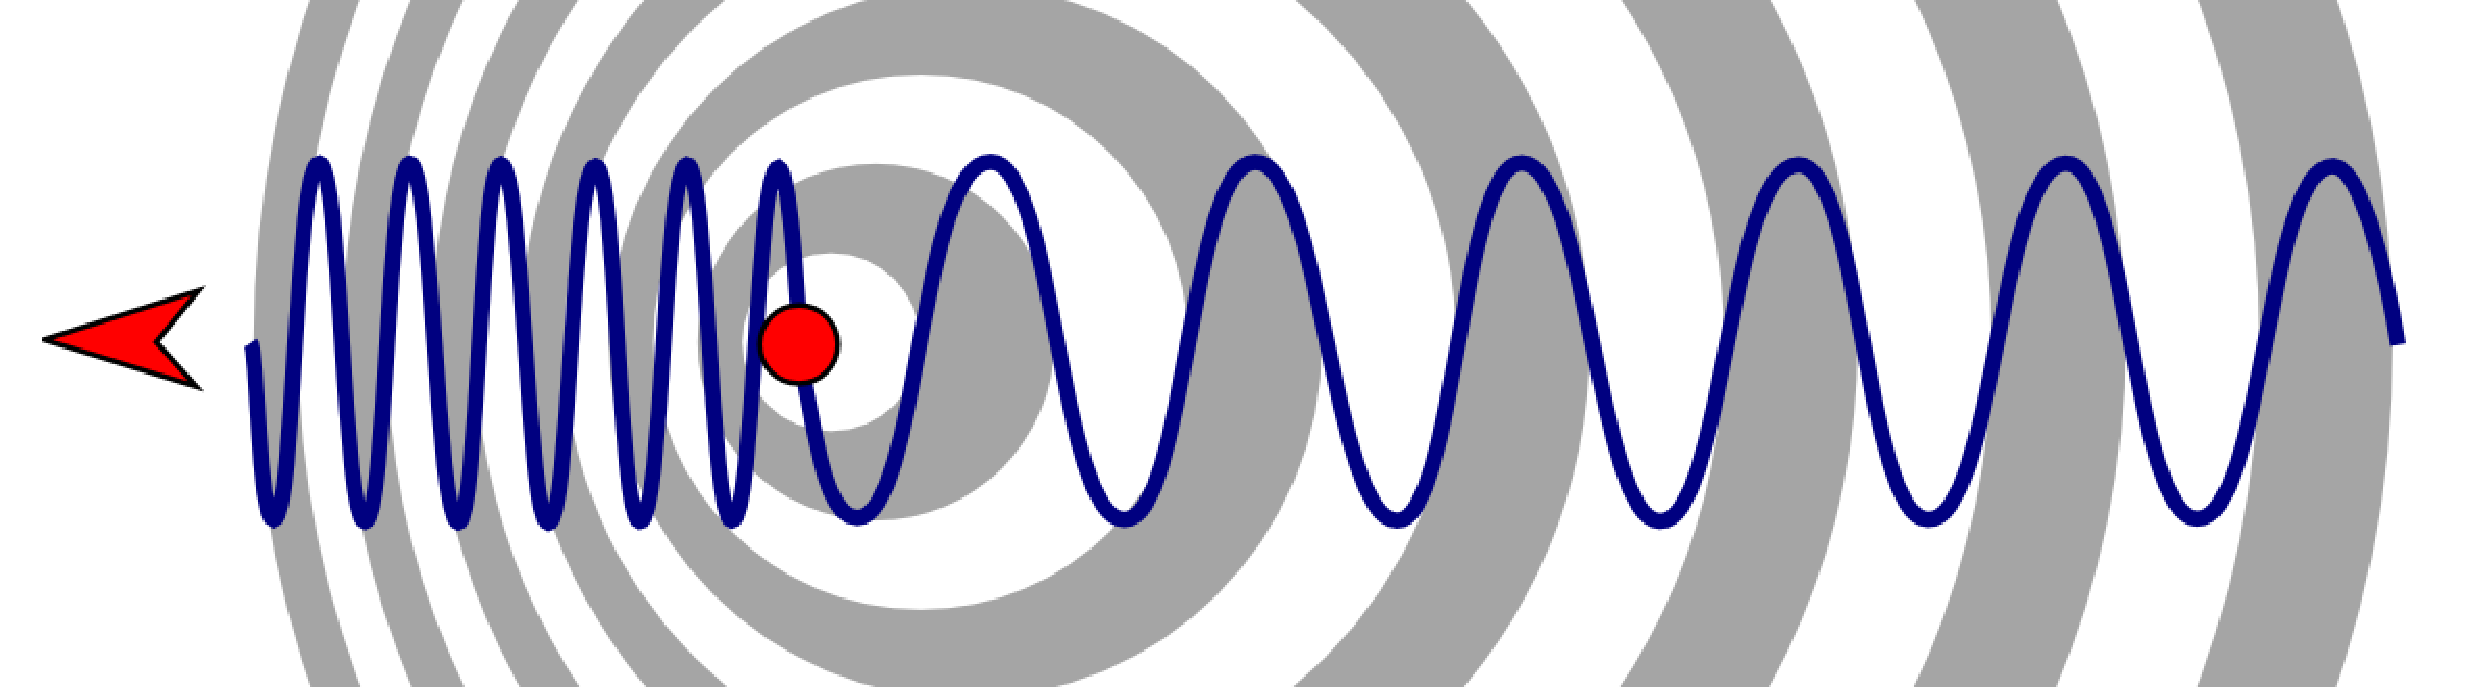
\includegraphics[width=0.5\textwidth]{doppler-ef}
\caption{Эффект Доплера}\label{doppler-ef}
\end{figure}

Формулу для релятивистского эффекта Доплера выводят из уравнений  специальной теории относительности и обусловлена она двумя причинами:
\begin{enumerate}
\item Классический аналог изменения частоты при относительном движении источника и приёмника.
\item Релятивистское замедление времени.
\end{enumerate}

Записывается он следующим образом:
\begin{equation}
\nu=\nu_0\cdot\frac{\sqrt{1-\frac{v^2}{c^2}}}{1-\frac{v}{c}\cdot\cos\theta},
\end{equation}
где $\nu$--- частота, с которой наблюдатель принимает волны, $\nu_0$ --- частота, с которой источник испускает волны, $v$ --- скорость источника, $\theta$ --- угол между направлением на источник и вектором скорости в системе отсчёта приёмника. 

Если источник радиально удаляется от наблюдателя, то $\theta =0$, если приближается, то $\theta =\pi$.

\textit{Красное смещение} --- сдвиг спектральных линий химических элементов в красную (длинноволновую) сторону. Оно показывает скорость удаления и расстояние до галактик или других объектов. Параметр красного смещения определяется таким образом:
\begin{equation}
z=\frac{\lambda-\lambda_0}{\lambda_0},
\end{equation}
где $\lambda$ и $\lambda _{0}$ --- значения длины волны в точках наблюдения и испускания излучения соответственно.

Доплеровское смещение длины волны в спектре источника, движущегося с лучевой скоростью $v_{r}$ и полной скоростью $v$, равно:
\begin{equation}
z_D=\frac{1+\frac{v_r}{c}}{\sqrt{1-\left(\frac{v}{c}\right)^2}}
\end{equation}

\textit{Гравитационное красное смещение} --- проявление эффекта изменения частоты испущенного некоторым источником света по мере удаления от массивных объектов, таких как звёзды и чёрные дыры; оно наблюдается как сдвиг спектральных линий в излучении источников, близких к массивным телам, в красную область спектра. Через длины волн и частоты записывается как:
\begin{equation}
Z_D=\frac{\lambda-\lambda_0}{\lambda_0}=\frac{\nu-\nu_0}{\nu_0}
\end{equation}

Также гравитационное красное смещение определяется из формулы, выведенной Эйнштейном:
\begin{equation}
Z_G=\frac{GM}{c^2r}-\frac{GM}{c^2R}\approx\frac{GM}{c^2r}, 
\end{equation}
т.к. $GM/c^2r\ll GM/c^2R$, где $M$ --- масса гравитирующего тела, $r$ --- радиальное расстояние от центра масс тела до точки излучения, $R$ ---  радиальное расстояние от центра масс тела до точки наблюдения.

\end{document}